%==============================================================================
% TutorAI — M.Tech Thesis Report
%
% HOW TO COMPILE (any standard TeX Live / MiKTeX install, or Overleaf pdfLaTeX):
%   pdflatex thesis.tex
%   pdflatex thesis.tex     % run twice so the TOC / references resolve
%
% The bibliography is embedded (thebibliography) so no .bib / bibtex is needed.
%
% BEFORE YOU SUBMIT, search for  \todoph  and fill each placeholder:
%   - your USN, the academic year, guide's designation
%   - publication details (once the conference paper is accepted)
%   - plagiarism-report similarity figure
% Everything in the body describes the real system in this repository.
%
% Screenshots: same four PNGs as the conference paper. The file looks in
% ./fig/ first and then ../fig/, so the copies used by tutorai.tex are found
% automatically. Missing images render as labelled placeholder boxes and never
% break the build.
%==============================================================================
\documentclass[12pt,a4paper,oneside]{report}

% ------------------------------ packages -------------------------------------
\usepackage[T1]{fontenc}
\usepackage[utf8]{inputenc}
\usepackage{mathptmx}                 % Times text + math (standard thesis font)
\usepackage[a4paper,left=3.5cm,right=2.5cm,top=2.5cm,bottom=2.5cm]{geometry}
\usepackage{setspace}
\usepackage{graphicx}
\usepackage{booktabs}
\usepackage{array}
\usepackage{url}
\usepackage{xcolor}
\usepackage{caption}
\usepackage{listings}
\usepackage{tikz}
\usetikzlibrary{positioning,arrows.meta,fit,backgrounds,shapes.geometric}
\usepackage{titlesec}
\usepackage[hidelinks]{hyperref}

\graphicspath{{fig/}{../fig/}}

% ------------------------------ styling --------------------------------------
\onehalfspacing
\setlength{\parskip}{4pt}

% Chapter headings: "CHAPTER 1" centred, then the title, both bold.
\titleformat{\chapter}[display]
  {\centering\bfseries\Large}
  {\MakeUppercase{\chaptertitlename}~\thechapter}
  {8pt}
  {\MakeUppercase}
\titlespacing*{\chapter}{0pt}{-10pt}{24pt}

\titleformat{\section}{\bfseries\large}{\thesection}{0.8em}{}
\titleformat{\subsection}{\bfseries\normalsize}{\thesubsection}{0.8em}{}

% ------------------------------ helpers --------------------------------------
% Fill-me-in placeholder, easy to search for.
\newcommand{\todoph}[1]{\textbf{[#1]}}

% Screenshot helper: shows the image if present, else a labelled placeholder box
% so the thesis always compiles.
\newcommand{\shot}[2][width=\linewidth]{%
  \IfFileExists{fig/#2}{\includegraphics[#1]{#2}}{%
    \IfFileExists{../fig/#2}{\includegraphics[#1]{#2}}{%
      \fbox{\parbox[c][45mm][c]{40mm}{\centering\small
        add screenshot:\\\texttt{fig/#2}}}}}}

% Listing style for JSON / code snippets.
\lstdefinestyle{code}{
  basicstyle=\ttfamily\small,
  breaklines=true,
  columns=fullflexible,
  showstringspaces=false,
  frame=single,
  framesep=4pt,
  xleftmargin=4pt,
  aboveskip=6pt,
  belowskip=6pt
}

% ------------------------------ metadata -------------------------------------
\newcommand{\thesistitle}{TutorAI: An Agentic, Validation-Gated Pipeline for
Self-Explaining, Highlight-Synchronized Visual Lessons on an Offline-First
Mobile Application}
\newcommand{\candidatename}{Subrath S}
\newcommand{\candidateusn}{\todoph{USN}}
\newcommand{\guidename}{Prasad A M}
\newcommand{\guidedesig}{\todoph{Designation, e.g.\ Assistant Professor}}
\newcommand{\deptname}{Department of Computer Science and Engineering}
\newcommand{\collegename}{Dayananda Sagar College of Engineering}
\newcommand{\collegecity}{Bangalore}
\newcommand{\university}{Visvesvaraya Technological University, Belagavi}
\newcommand{\academicyear}{\todoph{2025--2026}}

%==============================================================================
\begin{document}

% =============================== FRONT MATTER ================================
\pagenumbering{roman}

%============================== TITLE PAGE ====================================
\begin{titlepage}
\begin{center}
{\large \university\par}
\vspace{2mm}
\todoph{University logo here, if required: \texttt{\textbackslash includegraphics}}

\vspace{10mm}
{\normalsize A Thesis Report on\par}
\vspace{4mm}
{\Large\bfseries \thesistitle\par}

\vspace{10mm}
{\normalsize Submitted in partial fulfilment of the requirements for the award
of the degree of\par}
\vspace{3mm}
{\large\bfseries Master of Technology\par}
{\normalsize in\par}
{\large\bfseries Computer Science and Engineering\par}

\vspace{8mm}
{\normalsize Submitted by\par}
\vspace{2mm}
{\large\bfseries \candidatename\par}
{\normalsize USN: \candidateusn\par}

\vspace{8mm}
{\normalsize Under the guidance of\par}
\vspace{2mm}
{\large\bfseries \guidename\par}
{\normalsize \guidedesig\\ \deptname\par}

\vfill
\todoph{College logo here, if required}
\vspace{4mm}

{\normalsize\bfseries \deptname\\
\collegename\\
\collegecity\par}
\vspace{3mm}
{\normalsize Academic Year: \academicyear\par}
\end{center}
\end{titlepage}

%=============================== CERTIFICATE ==================================
\clearpage
\thispagestyle{plain}
\begin{center}
{\large\bfseries \collegename, \collegecity\\[1mm]
\deptname\par}
\vspace{10mm}
{\Large\bfseries CERTIFICATE\par}
\end{center}
\vspace{6mm}

This is to certify that the thesis entitled \emph{``\thesistitle''} is a
bonafide work carried out by \textbf{\candidatename} (USN: \candidateusn) in
partial fulfilment of the requirements for the award of the degree of
\textbf{Master of Technology in Computer Science and Engineering} of
\university\ during the academic year \academicyear. It is certified that all
corrections and suggestions indicated during the internal assessment have been
incorporated in the report. The thesis has been approved as it satisfies the
academic requirements in respect of the project work prescribed for the said
degree.

\vspace{20mm}
\noindent
\begin{tabular}{@{}p{0.48\textwidth}p{0.48\textwidth}@{}}
\textbf{\guidename} & \textbf{\todoph{HoD name}}\\
\guidedesig & Professor and Head\\
\deptname & \deptname\\
\collegename & \collegename\\
\end{tabular}

\vspace{18mm}
\noindent\textbf{External Viva}

\vspace{6mm}
\noindent
\begin{tabular}{@{}p{0.48\textwidth}p{0.48\textwidth}@{}}
Name of the Examiners & Signature with Date\\[12mm]
1. \rule{0.35\textwidth}{0.4pt} & \rule{0.35\textwidth}{0.4pt}\\[8mm]
2. \rule{0.35\textwidth}{0.4pt} & \rule{0.35\textwidth}{0.4pt}\\
\end{tabular}

%=============================== DECLARATION ==================================
\clearpage
\thispagestyle{plain}
\begin{center}
{\Large\bfseries DECLARATION\par}
\end{center}
\vspace{6mm}

I, \textbf{\candidatename} (USN: \candidateusn), student of Master of
Technology in Computer Science and Engineering, \collegename, \collegecity,
hereby declare that the thesis entitled \emph{``\thesistitle''} has been
carried out by me under the guidance of \textbf{\guidename}, \guidedesig,
\deptname, \collegename, and submitted in partial fulfilment of the
requirements for the award of the degree of Master of Technology in Computer
Science and Engineering of \university\ during the academic year
\academicyear. This thesis is my original work and, to the best of my
knowledge, it has not been submitted in part or in full for the award of any
other degree of any university.

\vspace{25mm}
\noindent Place: \collegecity\hfill \textbf{\candidatename}\\
Date: \rule{3cm}{0.4pt}\hfill USN: \candidateusn

%================================ ABSTRACT ====================================
\clearpage
\thispagestyle{plain}
\addcontentsline{toc}{chapter}{Abstract}
\begin{center}
{\Large\bfseries ABSTRACT\par}
\end{center}
\vspace{4mm}

A learner who wants a quick visual answer to ``how does this work'' usually has
to stitch together text from one source, a static picture from another, and a
separate video from a third. This thesis presents \textbf{TutorAI}, a complete,
working system that turns a single typed topic into a short lesson that
explains itself. Each lesson consists of three tightly coupled parts: a vector
diagram (SVG) whose meaningful parts carry stable, semantic identifiers; a
narration script split into ordered segments, where every segment names the
diagram parts it talks about; and one synthesized speech clip per segment with
a precisely measured duration. On an Android device, playback highlights the
referenced diagram parts while the matching audio plays, recreating the
``point and explain'' behaviour of a human tutor. Once downloaded, a lesson
replays fully offline and is kept in an on-device history.

The central engineering challenge is reliability: a large language model will
happily write narration that references a diagram part that does not exist,
which silently breaks the highlighting. TutorAI solves this with an agentic
generation pipeline built on LangGraph that separates planning, drawing,
critique-and-refine of the drawing, narration, and validation into distinct
nodes, and places a deterministic, non-LLM validator as a hard gate in front
of the cache: a lesson is never stored unless its SVG is well formed and every
referenced identifier really exists. Bounded refine and repair loops raise
quality while capping cost and latency. The backend is a stateless FastAPI
service with a shared, topic-keyed lesson cache, so a popular topic is
generated once and then served instantly. Both the LLM (Gemini) and the
text-to-speech engine sit behind swappable provider adapters, making model
choice a configuration concern. The Android client follows Clean Architecture
with MVVM, uses Room and a private file store for offline persistence, and
drives segment-synchronized highlighting through a WebView-hosted SVG and
ExoPlayer playlist.

The realized system was verified end to end: live generation produced a valid,
narrated, highlight-consistent lesson; the validation gate was shown to reject
and repair broken lessons; a hermetic suite of 48 key-free backend tests runs
in continuous integration; and the containerized backend and installable
Android build are produced by automated pipelines. The thesis describes the
methodology, architecture, implementation, and verified results, and discusses
limitations and future work including formal learning-outcome studies.

\vspace{6mm}
\noindent\textbf{Keywords:} generative AI, large language models, LLM agents,
intelligent tutoring systems, multimedia learning, SVG generation,
text-to-speech, FastAPI, LangGraph, Android, offline-first, software
architecture.

%============================== ACKNOWLEDGMENT ================================
\clearpage
\thispagestyle{plain}
\addcontentsline{toc}{chapter}{Acknowledgment}
\begin{center}
{\Large\bfseries ACKNOWLEDGMENT\par}
\end{center}
\vspace{4mm}

The satisfaction that accompanies the successful completion of any task would
be incomplete without the mention of the people who made it possible, whose
constant guidance and encouragement crowned the effort with success.

I express my sincere gratitude to my guide, \textbf{\guidename},
\guidedesig, \deptname, \collegename, for the valuable guidance, constant
encouragement, and constructive criticism extended throughout the course of
this project work.

I am grateful to \textbf{\todoph{HoD name}}, Professor and Head,
\deptname, \collegename, for the support and for providing the facilities
required to carry out this work.

I thank \textbf{\todoph{Principal name}}, Principal, \collegename, for
providing an excellent academic environment.

I also thank all the teaching and non-teaching staff of the \deptname\ for
their timely help, and my family and friends for their patience and
encouragement during the course of this work.

\vspace{12mm}
\hfill\textbf{\candidatename}


% ------------------------------ contents -------------------------------------
\tableofcontents

\clearpage
\addcontentsline{toc}{chapter}{List of Tables}
\listoftables

\clearpage
\addcontentsline{toc}{chapter}{List of Figures}
\listoffigures

%==================== LIST OF ABBREVIATIONS AND SYMBOLS =======================
\clearpage
\thispagestyle{plain}
\addcontentsline{toc}{chapter}{List of Abbreviations and Symbols}
\begin{center}
{\Large\bfseries LIST OF ABBREVIATIONS AND SYMBOLS\par}
\end{center}
\vspace{4mm}

\begin{center}
\begin{tabular}{@{}ll@{}}
\toprule
\textbf{Abbreviation} & \textbf{Expansion}\\
\midrule
AI    & Artificial Intelligence\\
API   & Application Programming Interface\\
APK   & Android Package Kit\\
CI/CD & Continuous Integration / Continuous Delivery\\
CSS   & Cascading Style Sheets\\
DAO   & Data Access Object\\
DI    & Dependency Injection\\
DTO   & Data Transfer Object\\
ER    & Entity--Relationship\\
FR    & Functional Requirement\\
HTTP(S) & Hypertext Transfer Protocol (Secure)\\
ITS   & Intelligent Tutoring System\\
JSON  & JavaScript Object Notation\\
LLM   & Large Language Model\\
LoC   & Lines of Code\\
MVVM  & Model--View--ViewModel\\
NFR   & Non-Functional Requirement\\
PCM   & Pulse-Code Modulation\\
REST  & Representational State Transfer\\
SDK   & Software Development Kit\\
SDLC  & Software Development Life Cycle\\
SSE   & Server-Sent Events\\
SVG   & Scalable Vector Graphics\\
TTS   & Text-to-Speech\\
UI    & User Interface\\
UML   & Unified Modeling Language\\
URL   & Uniform Resource Locator\\
WAV   & Waveform Audio File Format\\
XML   & Extensible Markup Language\\
\bottomrule
\end{tabular}
\end{center}

\vspace{6mm}
\noindent\textbf{Symbols}
\begin{center}
\begin{tabular}{@{}ll@{}}
\toprule
\textbf{Symbol} & \textbf{Meaning}\\
\midrule
$d_i$ & Measured duration (ms) of the audio clip of segment $i$\\
$D$   & Total lesson duration, $D=\sum_i d_i$\\
$R$   & Maximum repair retries (bounded loop budget)\\
$K$   & Maximum critique-and-refine passes\\
\bottomrule
\end{tabular}
\end{center}


% ================================ CHAPTERS ====================================
\clearpage
\pagenumbering{arabic}

%==============================================================================
\chapter{Introduction}
\label{ch:intro}
%==============================================================================

\section{Overview}
\label{sec:overview}

Good explanations are often visual and spoken at the same time. A teacher
points at a part of a drawing and says what it does; the pointing and the
talking happen together, so the listener never has to guess which part the
words are about. Most digital learning tools lose this link. A page of text
sits next to a fixed picture, and a video lives somewhere else. The learner
carries the load of connecting them.

This thesis describes \textbf{TutorAI}, a working end-to-end system that
rebuilds this ``point and explain'' experience automatically. The learner
types a single topic --- for example, \emph{Photosynthesis} --- into an
Android application. The system returns a self-contained \emph{lesson} made of
three parts:

\begin{enumerate}
  \item a diagram drawn as Scalable Vector Graphics (SVG) in which every
        meaningful visual element carries a stable, semantic identifier such
        as \texttt{sun}, \texttt{leaf}, or \texttt{chloroplast};
  \item a narration script split into ordered \emph{segments}, where each
        segment consists of a sentence or two of explanation together with the
        list of SVG element identifiers it talks about; and
  \item one synthesized speech clip per segment, produced by a text-to-speech
        (TTS) engine, with a precisely measured duration.
\end{enumerate}

During playback on the device, the current segment's audio plays while the SVG
elements it references are visually highlighted (a glow-and-scale emphasis),
so the learner always sees exactly what is being described. When the segment's
clip finishes, the highlight moves on with the narration. Because every asset
of a lesson is downloaded once and stored on the device, a saved lesson
replays fully offline, and an on-device history lets the learner revisit any
past topic.

The system consists of two cooperating applications. The \emph{backend} is a
stateless Python FastAPI service that hosts an agentic generation pipeline
built with LangChain and LangGraph. The pipeline orchestrates a Gemini large
language model (LLM) for planning, drawing, and narration, and a Gemini speech
model for audio, both hidden behind swappable provider adapters. Generated
lessons are cached under a normalized topic key so that a popular topic is
generated once and afterwards served instantly and cheaply. The \emph{client}
is a Kotlin Android application built with Jetpack Compose, following Clean
Architecture and the Model--View--ViewModel (MVVM) pattern, with Room and a
private file store for offline persistence and ExoPlayer for per-segment audio
playback.

The intellectual core of the work is not any single model but an
\emph{architectural} answer to a reliability problem: an LLM will happily
write narration that points at a diagram part that does not exist, which
silently breaks the highlighting that the whole product depends on. TutorAI
therefore splits generation into a graph of small steps with bounded
critique-and-refine and repair loops, and places a deterministic, non-LLM
validator as a hard gate in front of the cache. A lesson is never stored
unless its SVG is well formed and every identifier referenced by every
segment actually exists in the drawing.

\section{Problem Statement}
\label{sec:problem}

Learners who want a quick, visual explanation of a concept currently have to
stitch together text, static diagrams, and separately produced videos. There
is no lightweight tool where the user types a topic and immediately receives a
\emph{purpose-built diagram that explains itself} --- narrated, with the
relevant parts of the diagram lighting up exactly as they are discussed ---
and that can be revisited later without a network connection.

Building such a tool with generative AI raises four concrete technical
problems that this thesis addresses:

\begin{enumerate}
  \item \textbf{Cross-artifact consistency.} The diagram, the narration, and
        the audio are generated by different (probabilistic) steps, yet the
        product depends on an exact correspondence between narration
        references and diagram element identifiers. A single hallucinated
        identifier breaks synchronized highlighting.
  \item \textbf{Deterministic audio--visual synchronization.} Highlighting
        must stay aligned with speech on a mobile device, offline, without
        streaming timing data or word-level alignment infrastructure.
  \item \textbf{Cost and latency of generation.} Cold generation requires
        several LLM calls plus per-segment speech synthesis. Repeated requests
        for the same topic must not repeat this cost, and unbounded
        self-correction loops must not inflate it.
  \item \textbf{Reproducible engineering.} The system must be testable without
        live AI keys, deployable as a container, and resilient to externally
        controlled details such as hosted model identifiers changing over
        time.
\end{enumerate}

\section{Objectives}
\label{sec:objectives}

The objectives of this project work are:

\begin{enumerate}
  \item To design and implement an \textbf{agentic generation pipeline}
        (LangGraph state graph) that transforms a free-text topic into a
        validated lesson: an SVG diagram with stable semantic identifiers,
        ordered narration segments that reference only existing identifiers,
        and per-segment TTS audio with measured durations.
  \item To design a \textbf{deterministic, non-LLM validation gate} with
        bounded repair and critique-and-refine loops, guaranteeing that no
        lesson whose narration references a non-existent diagram element is
        ever cached or served.
  \item To implement a \textbf{stateless FastAPI backend} with an
        asynchronous job model, a shared topic-keyed lesson cache with request
        coalescing, an asset store, and swappable LLM/TTS provider adapters.
  \item To implement an \textbf{offline-first Android client} (Kotlin,
        Jetpack Compose, Clean Architecture + MVVM) that generates lessons via
        job polling, plays them with segment-synchronized SVG highlighting,
        and persists them (Room + file store) for fully offline replay with
        an on-device history.
  \item To apply sound \textbf{software-engineering practice} throughout:
        documented UML-first design, classical design patterns at the seams,
        hermetic key-free automated tests, containerization, and CI/CD
        pipelines for both backend and client.
  \item To \textbf{verify the realized system} end to end against live
        models and report its behaviour honestly, distinguishing verified
        results from future evaluation.
\end{enumerate}

\section{Motivation}
\label{sec:motivation}

The motivation for this work is threefold.

\textbf{Pedagogical.} Decades of research on multimedia learning show that
people learn more deeply from words and pictures presented together than from
words alone, and that spoken narration synchronized with relevant graphics
reduces cognitive load compared to on-screen text (the modality and temporal
contiguity principles). Bloom's classic finding that one-to-one tutoring
dramatically outperforms group instruction has driven a long search for
scalable tutoring software. A tool that generates a narrated, self-pointing
diagram for \emph{any} typed topic, on demand, brings a small but genuinely
useful slice of that tutoring behaviour to anyone with a phone.

\textbf{Technical.} Large language models have made it possible to generate
explanations, structured data, and even vector graphics from a single prompt,
but they remain probabilistic: outputs may be malformed or internally
inconsistent. The recent literature on LLM agents proposes decomposition,
self-critique, and iterative repair as remedies, yet published systems rarely
need the \emph{hard} cross-artifact guarantee that TutorAI needs (every
narration reference must resolve to a real diagram element). Demonstrating
that a small state graph with bounded loops and a deterministic gate can make
a probabilistic generator reliable enough for a correctness-critical feature
is a useful, transferable engineering result.

\textbf{Practical.} Learners in many settings have intermittent or expensive
connectivity. An offline-first design --- download once, replay forever,
history on the device, no accounts, no personal data on the server --- makes
the tool usable and private in exactly the settings where lightweight learning
aids matter most. A stateless backend with a shared cache also keeps the
operating cost of such a service low: the marginal cost of a popular topic
tends towards zero.

\section{Organization of the Thesis}
\label{sec:organization}

The remainder of this thesis is organized as follows.
Chapter~\ref{ch:literature} surveys the relevant literature across
intelligent tutoring systems, multimedia learning theory, large language
models and agentic orchestration, automatic diagram generation, speech
synthesis, and offline-first mobile architecture, and identifies the research
gap. Chapter~\ref{ch:methodology} presents the methodology: the requirements,
the key design decisions, the agentic generation method with its validation
gate, the synchronization model, and the phased development and testing
process followed. Chapter~\ref{ch:design} details the design and
implementation of the backend and the Android client, including the domain
model, the API contract, the design patterns employed, and the CI/CD
pipelines. Chapter~\ref{ch:results} reports the verified results of the
realized system and discusses its behaviour, trade-offs, and limitations.
Chapter~\ref{ch:conclusion} concludes and outlines the future scope. The
appendices reproduce the API contract, the lesson manifest schema, and the
repository layout.

%==============================================================================
\chapter{Literature Survey}
\label{ch:literature}
%==============================================================================

This chapter surveys the six bodies of work that TutorAI draws on:
intelligent tutoring systems and AI in education; the cognitive theory of
learning from words and pictures; large language models as content
generators; agentic orchestration and self-correction of LLMs; automatic
diagram and vector-graphics generation; and speech synthesis together with
offline-first mobile architecture. Each section closes with the specific
lesson the surveyed work contributes to this thesis, and the chapter closes
with a summary table and the identified research gap.

%------------------------------------------------------------------------------
\section{Intelligent Tutoring Systems and AI in Education}
%------------------------------------------------------------------------------

The ambition of software that teaches is old and well studied. Bloom's
influential ``2 sigma'' finding --- that students taught one-to-one by a human
tutor performed about two standard deviations better than students in
conventional classrooms --- framed the field's goal: find scalable methods of
instruction as effective as individual tutoring~\cite{bloom1984}. Intelligent
Tutoring Systems (ITS) pursued this goal by modelling the domain, the student,
and pedagogy explicitly. Anderson \emph{et al.}'s cognitive tutors, grounded
in the ACT-R theory of cognition, demonstrated that model-tracing tutors could
achieve large learning gains in algebra and programming, and distilled a set
of pragmatic design lessons from a decade of classroom
deployment~\cite{anderson1995cognitive}. VanLehn's later meta-analysis
compared human tutoring, step-based ITS, and answer-based systems, and found
--- contrary to folklore --- that mature step-based tutoring systems were
nearly as effective as human tutors (effect sizes of roughly 0.76 versus
0.79)~\cite{vanlehn2011}. The catch has always been cost: classical ITS
require painstaking, per-domain knowledge engineering, which is why they
exist only for a handful of well-resourced subjects.

The arrival of large language models changed the economics of educational
content. Kasneci \emph{et al.} survey the opportunities and challenges of
LLMs such as ChatGPT in education: on the one hand personalized explanations,
instant feedback, and content generation at negligible marginal cost; on the
other hand hallucination, bias, over-reliance, and the difficulty of
verifying generated material~\cite{kasneci2023chatgpt}. This tension ---
generation is now cheap but \emph{trustworthy} generation is not --- is the
starting point of the present work.

\emph{Lesson for TutorAI.} TutorAI does not attempt a full ITS: it has no
student model and no adaptive curriculum. It automates one narrow, valuable
tutoring behaviour --- pointing at a drawing while explaining it --- for an
open set of topics, at near-zero marginal cost per repeated topic. Where a
classical ITS invests in hand-built domain knowledge, TutorAI invests in
\emph{verification} of machine-generated content.

%------------------------------------------------------------------------------
\section{Learning from Words and Pictures}
%------------------------------------------------------------------------------

Why insist on a diagram whose parts light up in time with speech, rather than
a paragraph of text? The answer comes from cognitive psychology. Paivio's
dual-coding theory holds that verbal and visual information are processed in
separate channels and that learning is stronger when both are
engaged~\cite{paivio1991}. Sweller's cognitive load theory adds that working
memory is sharply limited, so instruction should avoid forcing the learner to
hold and cross-reference disconnected representations~\cite{sweller1988}.

Mayer's cognitive theory of multimedia learning operationalizes these ideas
into evidence-backed design principles~\cite{mayer2014multimedia}. Three of
them read almost as a specification of TutorAI's player. The
\emph{multimedia principle}: people learn better from words and pictures than
from words alone. The \emph{modality principle}: spoken narration
accompanying a graphic beats on-screen text, because it spreads processing
across the auditory and visual channels. The \emph{temporal contiguity} and
\emph{signaling} principles: narration and the corresponding part of the
graphic should be presented at the same time, and the learner's attention
should be explicitly cued to the relevant part. Mayer and Moreno's survey of
ways to reduce cognitive load in multimedia learning names synchronized
narration-plus-highlighting as one of the most effective
techniques~\cite{mayermoreno2003}.

\emph{Lesson for TutorAI.} The product form --- segment-level narration,
each segment simultaneously highlighting exactly the diagram parts it
describes, with captions available --- is a direct implementation of the
multimedia, modality, temporal-contiguity, and signaling principles. This
grounding also explains why a \emph{broken} highlight (a narration segment
pointing at a non-existent part) is not a cosmetic bug but a destruction of
the pedagogical mechanism, and hence why the thesis treats reference
consistency as a hard correctness property.

%------------------------------------------------------------------------------
\section{Large Language Models for Content Generation}
%------------------------------------------------------------------------------

The transformer architecture~\cite{vaswani2017attention} and the subsequent
scaling of autoregressive language models established that a single
pre-trained model can perform diverse generation tasks from natural-language
instructions alone. Brown \emph{et al.} showed with GPT-3 that few-shot
prompting suffices for many tasks without task-specific
fine-tuning~\cite{brown2020gpt3}. The Gemini family extended this to natively
multimodal models spanning text, code, images, and audio, with ``Flash''-class
variants engineered for low latency and cost~\cite{gemini2023} --- the class
of model TutorAI uses for planning, drawing, narration, and repair. Beyond
prose, Chen \emph{et al.}'s Codex work demonstrated that LLMs trained on code
generate syntactically constrained, machine-interpretable artifacts with
useful reliability~\cite{chen2021codex}; generating SVG markup, as TutorAI
does, is essentially structured code generation. Liu \emph{et al.}
systematize prompting methods --- instruction design, output schemas,
temperature control --- as the practical interface for steering such
models~\cite{liu2023promptsurvey}.

Two properties of LLM generation matter for this thesis. First,
\emph{structured output}: modern APIs can constrain generation to a JSON
schema, which TutorAI uses for plans, narration segments, and repair
responses, validated by Pydantic on receipt. Second, \emph{hallucination}: Ji
\emph{et al.}'s survey documents that language models produce fluent content
untethered from their inputs across virtually all generation
tasks~\cite{ji2023hallucination}. Schema-constrained output fixes the
\emph{shape} of a response but not its \emph{referential truth}: narration can
be perfectly valid JSON and still reference the identifier
\texttt{mitochondria} when the drawing contains no such element.

For completeness, raster text-to-image models such as Stable
Diffusion~\cite{rombach2022stable} can also illustrate topics, but their
output is pixels: there are no addressable parts, so nothing can be
selectively highlighted, and no deterministic validator can check whether the
image matches the narration. This rules them out for TutorAI's purpose and
motivates vector output.

\emph{Lesson for TutorAI.} Use an LLM for what it is good at (planning,
drawing well-known concepts, fluent narration, structured JSON), but treat
referential consistency as a property to be \emph{checked deterministically},
never assumed.

%------------------------------------------------------------------------------
\section{LLM Agents, Orchestration, and Self-Correction}
%------------------------------------------------------------------------------

A second line of work addresses reliability by wrapping the model in a
\emph{process}. Chain-of-thought prompting showed that eliciting intermediate
reasoning steps improves accuracy on multi-step problems~\cite{wei2022cot}.
ReAct interleaved reasoning with tool-using actions, letting a model gather
facts and act on feedback~\cite{yao2023react}. Most directly relevant are the
self-correction methods: Self-Refine has the model critique and then improve
its own output iteratively~\cite{madaan2023selfrefine}; Reflexion converts
environment feedback into verbal self-reflections that improve subsequent
attempts~\cite{shinn2023reflexion}; and Chen \emph{et al.} teach models to
self-debug generated code against execution feedback~\cite{chen2023selfdebug}.
A consistent finding across these papers is that critique grounded in
\emph{concrete, externally produced error signals} (failing tests, parser
errors) outperforms free-form self-assessment.

Orchestration frameworks make such processes buildable. LangChain provides
the component model for prompts, models, and tools~\cite{langchain}, and
LangGraph structures an application as an explicit state graph --- typed
state flowing through nodes, with conditional edges for loops --- rather than
an open-ended autonomous loop~\cite{langgraph}. The graph form matters for
production systems: it makes control flow inspectable, each node separately
testable, and loop budgets explicit.

\emph{Lesson for TutorAI.} TutorAI adopts decomposition
(plan~$\to$~draw~$\to$~narrate), a bounded critique-and-refine loop for the
drawing, and a bounded repair loop driven by a validator's exact error list
--- the ``self-debugging with real feedback'' pattern. It deliberately
rejects open-ended agency: the graph is small, static, and every loop has a
configured budget, so worst-case cost and latency are capped. The novel
element relative to the surveyed work is that the final arbiter is not the
model's own judgement but a deterministic, non-LLM gate that enforces a
cross-artifact invariant before anything is cached.

%------------------------------------------------------------------------------
\section{Automatic Diagram and Vector-Graphics Generation}
%------------------------------------------------------------------------------

TutorAI needs drawings whose parts are \emph{addressable}. SVG, a W3C
standard, represents images as an XML document tree in which any element can
carry an \texttt{id} attribute and be styled or animated
individually~\cite{svgspec} --- precisely the property synchronized
highlighting requires, and one no raster format offers.

Prior work on generating vector graphics spans learned latent models and
direct code generation. DeepSVG learns a hierarchical generative network over
SVG path commands, targeting interpolation and animation of icon-scale
graphics~\cite{carlier2020deepsvg}. StarVector treats SVG as code and
generates it with a multimodal LLM from images or text, showing that
modern code models internalize the SVG grammar
well~\cite{rodriguez2023starvector}. General code-generation results
\cite{chen2021codex} support the same conclusion. However, none of these
systems constrain the \emph{semantics of identifiers}: they produce plausible
markup, not markup whose element ids form a contract with a separately
generated narration. Template- and grammar-based diagram tools (of which
Mermaid is a popular example) guarantee well-formedness by construction, but
only within a fixed diagram vocabulary (flowcharts, sequence diagrams), which
is too narrow for arbitrary educational topics like photosynthesis or the
water cycle.

\emph{Lesson for TutorAI.} Have the LLM draw free-form SVG (breadth), impose
an \emph{id contract} through prompting (every meaningful element gets a
semantic id; narration may reference only existing ids), and enforce the
contract with an XML parser rather than trusting the model (reliability).
Quality is then raised --- not guaranteed --- by the critique-and-refine
loop.

%------------------------------------------------------------------------------
\section{Speech Synthesis and Narrated Content}
%------------------------------------------------------------------------------

Neural TTS made synthesized narration acceptable for learning content.
WaveNet demonstrated autoregressive generation of raw audio waveforms with
naturalness far beyond concatenative systems~\cite{oord2016wavenet}, and
Tacotron~2 established the now-standard text~$\to$~mel-spectrogram~$\to$
vocoder pipeline achieving near-human mean opinion scores~\cite{shen2018tacotron2}.
Today, hosted TTS services (including Gemini's speech models) expose this
capability behind an API that returns audio for text.

The synchronization question --- how to keep visuals aligned with speech ---
is usually answered with word-level timestamps or forced alignment, which
requires either streaming infrastructure or per-word timing metadata, both
fragile on an offline mobile target. The alternative TutorAI adopts is
coarser but deterministic: synthesize one clip per narration segment,
\emph{measure} its exact duration from the PCM byte count and sample rate,
and drive highlighting from clip boundaries. Synchronization then requires no
timing data beyond what the device player already knows (which clip is
playing), and it survives offline replay trivially.

\emph{Lesson for TutorAI.} Segment-level synchronization trades pointer
granularity for determinism and offline robustness --- an explicit,
defensible design decision grounded in the target environment.

%------------------------------------------------------------------------------
\section{Offline-First Mobile Applications and Software Architecture}
%------------------------------------------------------------------------------

Offline-first design treats the network as an enhancement rather than a
prerequisite: applications keep a complete local copy of the data they need
and synchronize opportunistically~\cite{offlinefirst}. For a learning tool
aimed partly at users with intermittent connectivity, this is a requirement,
not a preference. On Android, Google's architecture guidance recommends a
layered structure --- UI, domain, and data layers with unidirectional data
flow and reactive state~\cite{androidguide} --- which TutorAI follows using
Jetpack Compose, ViewModels exposing immutable state via \texttt{StateFlow},
Room for structured storage, and a private file store for binary assets.

At the level of software structure, Martin's Clean Architecture argues for
dependency inversion: business rules at the centre, frameworks and I/O at the
edges, boundaries crossed through interfaces~\cite{martin2017clean}. The
classical design-patterns catalogue~\cite{gamma1994} supplies the vocabulary
TutorAI uses at its seams --- Strategy, Abstract Factory, Adapter, Builder,
Facade, Repository --- and the Twelve-Factor App methodology supplies the
operational discipline of strict configuration-through-environment
\cite{twelvefactor}, which is what lets the same codebase run on mock
providers in tests and real Gemini providers in production, and lets hosted
model identifiers be pinned in configuration rather than code.

\emph{Lesson for TutorAI.} None of these practices is novel individually;
the survey point is that an AI-centred system still succeeds or fails on
ordinary architectural discipline. The provider adapters, hermetic tests, and
configuration-first design described in Chapters~\ref{ch:methodology}
and~\ref{ch:design} are direct applications of this literature.

%------------------------------------------------------------------------------
\section{Summary and Research Gap}
%------------------------------------------------------------------------------

Table~\ref{tab:litsummary} condenses the survey.

\begin{table}[htbp]
\caption{Summary of the literature surveyed and its role in this thesis}
\label{tab:litsummary}
\centering
\small
\renewcommand{\arraystretch}{1.3}
\begin{tabular}{@{}p{0.26\textwidth}p{0.30\textwidth}p{0.34\textwidth}@{}}
\toprule
\textbf{Area (key works)} & \textbf{Established result} & \textbf{Use in TutorAI}\\
\midrule
ITS / AI in education
\cite{bloom1984,anderson1995cognitive,vanlehn2011,kasneci2023chatgpt}
& Tutoring software works but classical ITS need costly per-domain
engineering; LLMs make content cheap but unverified.
& Automate one tutoring behaviour (point-and-explain) for open topics;
invest in verification instead of hand-built domain knowledge.\\
Multimedia learning
\cite{paivio1991,sweller1988,mayer2014multimedia,mayermoreno2003}
& Synchronized narration + signaled graphics measurably improve learning.
& Defines the product form; makes reference consistency a hard
correctness property.\\
LLMs for generation
\cite{vaswani2017attention,brown2020gpt3,gemini2023,chen2021codex,liu2023promptsurvey,ji2023hallucination}
& LLMs generate prose, code, and structured data well, but hallucinate;
schemas fix shape, not referential truth.
& Gemini via adapters; structured-output prompts; motivates the
deterministic gate.\\
Agents / self-correction
\cite{wei2022cot,yao2023react,madaan2023selfrefine,shinn2023reflexion,chen2023selfdebug,langchain,langgraph}
& Decomposition and critique on concrete error signals improve
reliability; graphs make agent control flow explicit.
& LangGraph pipeline; bounded critique-and-refine; repair loop fed by
validator errors.\\
Vector-graphics generation
\cite{svgspec,carlier2020deepsvg,rodriguez2023starvector,rombach2022stable}
& LLMs can write SVG; raster models offer no addressable parts; grammar
tools are narrow.
& Free-form LLM-drawn SVG under a prompted id contract, enforced by an
XML parser.\\
TTS \cite{oord2016wavenet,shen2018tacotron2}
& Neural TTS is natural enough for narration; word-level sync needs
fragile timing data.
& Per-segment clips with byte-measured durations; segment-level sync.\\
Mobile / architecture
\cite{offlinefirst,androidguide,martin2017clean,gamma1994,twelvefactor}
& Offline-first, layered architecture, patterns, and 12-factor config are
proven practice.
& Clean Architecture + MVVM client; provider adapters; hermetic key-free
tests; container + CI/CD.\\
\bottomrule
\end{tabular}
\end{table}

\textbf{Research gap.} Each ingredient above exists in isolation: LLMs that
draw SVG, agent frameworks with self-correction, multimedia-learning theory
prescribing synchronized narration, and offline-first mobile practice. What
the surveyed literature does not provide is a system that \emph{combines}
them under a hard cross-artifact consistency guarantee --- narration that is
machine-checked, before caching, to reference only diagram elements that
exist --- delivered end to end on an offline-first mobile client with
deterministic audio--visual synchronization. Published self-correction work
validates outputs against tests or environments for a \emph{single} artifact;
TutorAI's gate validates the \emph{joint} consistency of two independently
generated artifacts (drawing and narration) and refuses service rather than
degrade. Closing that gap --- and demonstrating it with a verified, tested,
deployable implementation --- is the contribution of this thesis.

%==============================================================================
\chapter{Methodology}
\label{ch:methodology}
%==============================================================================

This chapter presents the methodology of the work: the requirements that
define the problem precisely (Section~\ref{sec:requirements}), the three
locked design decisions that shape the whole system
(Section~\ref{sec:decisions}), the agentic generation method with its
deterministic validation gate (Section~\ref{sec:genmethod}), the
synchronization model (Section~\ref{sec:syncmethod}), the caching and
idempotency strategy (Section~\ref{sec:cachemethod}), and the phased
development and testing process followed (Section~\ref{sec:sdlc}).

%------------------------------------------------------------------------------
\section{Requirements Analysis}
\label{sec:requirements}
%------------------------------------------------------------------------------

\subsection{Target Users and User Stories}

The system targets three user groups: students revising a concept,
self-learners exploring an unfamiliar topic, and educators generating quick
visual aids. The core user stories are listed in Table~\ref{tab:stories}.

\begin{table}[htbp]
\caption{Core user stories}
\label{tab:stories}
\centering
\small
\renewcommand{\arraystretch}{1.3}
\begin{tabular}{@{}lp{0.14\textwidth}p{0.34\textwidth}p{0.30\textwidth}@{}}
\toprule
\textbf{Id} & \textbf{As a\ldots} & \textbf{I want to\ldots} & \textbf{So that\ldots}\\
\midrule
US-1 & learner & type a topic and get a narrated diagram & I understand it visually and aurally\\
US-2 & learner & see diagram parts highlight as they are explained & I know exactly what is being described\\
US-3 & learner & pause, resume, and replay any segment & I can learn at my own pace\\
US-4 & learner & find all my past topics in a history list & I can revisit lessons\\
US-5 & learner & replay a saved lesson with no internet & I can study offline\\
US-6 & learner & retry generation if a result is poor & I get a usable lesson\\
\bottomrule
\end{tabular}
\end{table}

\subsection{Functional Requirements}

\begin{description}
  \item[FR-1] Accept a free-text topic from the user.
  \item[FR-2] Generate an SVG diagram with stable, semantic element
        identifiers.
  \item[FR-3] Generate an ordered narration script split into segments, each
        referencing the SVG element identifiers it describes.
  \item[FR-4] Produce one TTS audio clip per segment with a measured
        duration.
  \item[FR-5] Assemble a self-contained lesson manifest (SVG + segments +
        audio references + durations).
  \item[FR-6] Serve cached lessons for previously requested topics.
  \item[FR-7] On device: download and persist the full lesson (manifest +
        assets) locally.
  \item[FR-8] On device: play the lesson, highlighting each segment's SVG
        element identifiers while its audio plays.
  \item[FR-9] On device: provide play, pause, resume, seek-by-segment, and
        replay controls.
  \item[FR-10] On device: maintain a searchable history of saved lessons.
  \item[FR-11] On device: replay any saved lesson fully offline.
  \item[FR-12] Surface clear errors and allow regeneration on failure.
\end{description}

\subsection{Non-Functional Requirements}

\begin{table}[htbp]
\caption{Non-functional requirements}
\label{tab:nfr}
\centering
\small
\renewcommand{\arraystretch}{1.3}
\begin{tabular}{@{}llp{0.62\textwidth}@{}}
\toprule
\textbf{Id} & \textbf{Category} & \textbf{Requirement}\\
\midrule
NFR-1 & Performance & Cache hit returns a manifest in under 500\,ms; cold
generation target under 30\,s\\
NFR-2 & Offline & Saved lessons play with zero network calls\\
NFR-3 & Reliability & Generation validates SVG well-formedness and identifier
consistency before caching\\
NFR-4 & Cost & Identical topics are generated once and shared via cache\\
NFR-5 & Portability & LLM and TTS providers are swappable behind adapters\\
NFR-6 & Maintainability & Clear layering, documented design patterns,
unit-testable core\\
NFR-7 & Privacy & No accounts; personal history never leaves the device\\
NFR-8 & Accessibility & Captions shown; adjustable playback; readable
contrast\\
\bottomrule
\end{tabular}
\end{table}

\subsection{Scope Exclusions (Version 1)}

User accounts and cross-device cloud synchronization, editing or annotating
generated diagrams, a multi-language user interface (lesson language is a
parameter, but the UI is single-language), social and sharing features, and
real-time word-level highlighting (segment-level synchronization is used, as
motivated in Section~\ref{sec:syncmethod}) are explicitly out of scope.

%------------------------------------------------------------------------------
\section{Key Design Decisions}
\label{sec:decisions}
%------------------------------------------------------------------------------

Three decisions, taken early and documented before implementation, shape
everything else in the system.

\textbf{Decision 1: Synchronization by pre-rendered timed segments.} Rather
than align voice to highlight at play time, the server splits the narration
into segments, renders one audio clip per segment, and \emph{measures} each
clip's duration. The device simply plays the clips in order and highlights
the parts named by the current clip. This makes synchronization deterministic
and removes any need for the network during playback (NFR-2), at the cost of
segment-level rather than word-level pointer granularity.

\textbf{Decision 2: Stateless backend with a shared cache.} There are no user
accounts on the server (NFR-7). Lessons are cached under a normalized topic
key, so a popular topic is generated once and then served to everyone
(NFR-1, NFR-4). Statelessness keeps the server trivially scalable and simple
to reason about; all personal state (history) lives on the device.

\textbf{Decision 3: Provider adapters.} The language model and the speech
engine sit behind narrow interfaces; the pipeline talks to those interfaces
and never to a vendor SDK directly (NFR-5). Choosing a model --- or replacing
the vendor entirely --- is a configuration change. This also acknowledges an
operational reality: hosted model identifiers change over time, so the model
name is treated as configuration, verified against the live API by a small
helper tool, and pinned in settings rather than in code.

%------------------------------------------------------------------------------
\section{The Agentic Generation Method}
\label{sec:genmethod}
%------------------------------------------------------------------------------

\subsection{Why a Graph and Not a Single Prompt}

A single mega-prompt (``produce a diagram, narration, and timing for topic
X'') couples all failure modes together: if any part of the output is
malformed, the whole response must be regenerated, and there is no precise
error signal to steer the retry. Decomposing generation into a
\emph{state graph} of small steps gives three properties the product needs:

\begin{enumerate}
  \item each artifact (plan, drawing, narration) can be \emph{validated and
        repaired in isolation}, with concrete error messages;
  \item each node is independently testable against mock providers; and
  \item deterministic steps (validation, TTS rendering, assembly) are
        separated from probabilistic ones, so reliability mechanisms attach
        exactly where the risk is.
\end{enumerate}

The pipeline is implemented as a LangGraph \texttt{StateGraph}: a single
typed state object flows through nodes connected by conditional edges. The
graph is small, static, and every loop carries a configured budget --- this
is deliberate rejection of open-ended agent autonomy in favour of an
inspectable, bounded process.

\subsection{Pipeline Stages}

Figure~\ref{fig:pipeline} shows the graph. Its nodes are:

\begin{figure}[htbp]
\centering
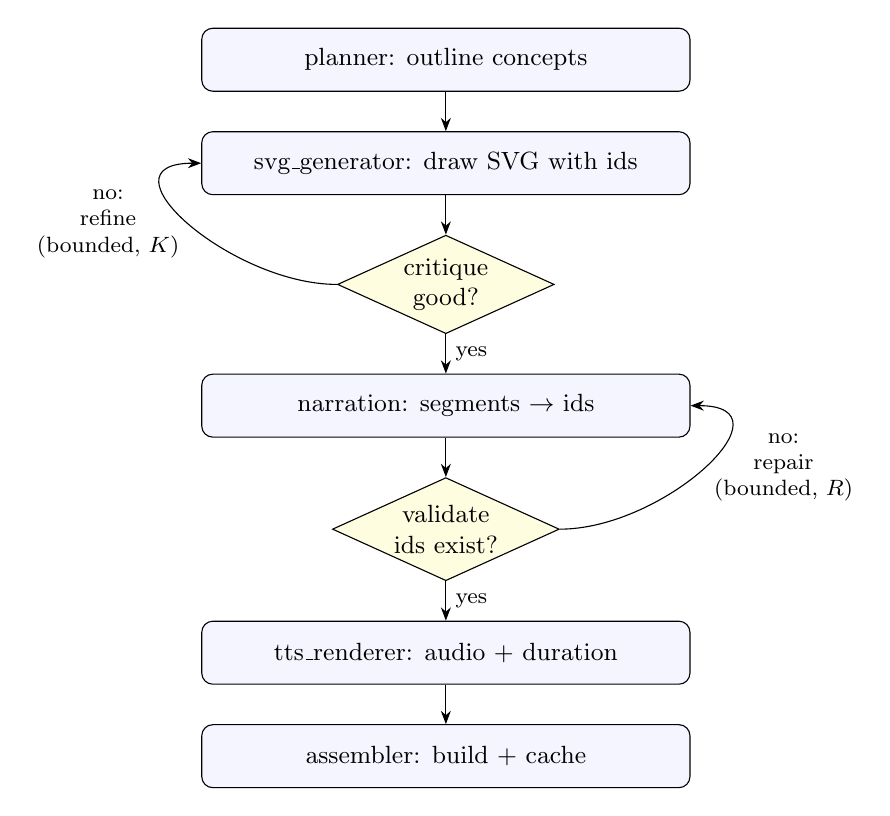
\begin{tikzpicture}[
  font=\small,
  node distance=5mm,
  n/.style={draw, rounded corners, align=center, minimum width=62mm,
            minimum height=8mm, fill=blue!4},
  d/.style={draw, diamond, aspect=2.2, align=center, inner sep=1pt,
            fill=yellow!12},
  >={Stealth}
]
\node[n] (plan) {planner: outline concepts};
\node[n, below=of plan] (svg) {svg\_generator: draw SVG with ids};
\node[d, below=of svg] (crit) {critique\\good?};
\node[n, below=of crit] (narr) {narration: segments $\rightarrow$ ids};
\node[d, below=of narr] (val) {validate\\ids exist?};
\node[n, below=of val] (tts) {tts\_renderer: audio + duration};
\node[n, below=of tts] (asm) {assembler: build + cache};

\draw[->] (plan) -- (svg);
\draw[->] (svg) -- (crit);
\draw[->] (crit) -- node[right,font=\footnotesize]{yes} (narr);
\draw[->] (narr) -- (val);
\draw[->] (val) -- node[right,font=\footnotesize]{yes} (tts);
\draw[->] (tts) -- (asm);

\draw[->] (crit.west) to[out=180,in=180,looseness=1.5]
  node[left,font=\footnotesize,align=center]{no:\\refine\\(bounded, $K$)} (svg.west);
\draw[->] (val.east) to[out=0,in=0,looseness=1.5]
  node[right,font=\footnotesize,align=center]{no:\\repair\\(bounded, $R$)} (narr.east);
\end{tikzpicture}
\caption{The generation graph. A bounded critique-and-refine loop improves
the drawing before narration is written; a bounded repair loop fixes
narration that fails the deterministic validator. A lesson reaches the
assembler only after it passes validation.}
\label{fig:pipeline}
\end{figure}

\begin{description}
  \item[Planner.] The model outlines the concepts and a visual plan for the
        topic. Planning once, up front, keeps the drawing and the narration
        aligned to the same concept set.
  \item[SVG generator.] Given the plan, the model draws the SVG and assigns a
        semantic \texttt{id} to every meaningful part (for example
        \texttt{sun}, \texttt{leaf}, \texttt{chloroplast}). The prompt
        instructs the model to return \emph{only} SVG.
  \item[Critique and refine.] A critique step scores the drawing and lists
        concrete problems. If the score is below a threshold and budget
        remains, a refine step redraws with that feedback and the critique
        runs again, up to $K$ passes. If the budget runs out, the best
        drawing so far is accepted. This is a focused application of the
        self-refine idea~\cite{madaan2023selfrefine}, applied only to the
        artifact that benefits most.
  \item[Narration generator.] Given the \emph{finished} drawing, the model
        writes ordered narration as schema-constrained JSON: each segment has
        text and a list of element identifiers. Writing narration against the
        real drawing steers the model toward referencing parts that exist ---
        but does not guarantee it, which is why the next node exists.
  \item[Validator.] This node uses no model (Section~\ref{sec:gate}).
  \item[Repair.] If validation fails and retries remain (budget $R$), the
        repair step receives the \emph{exact} list of offending identifiers
        and parse errors and is asked for the minimal correction; validation
        then runs again. If the budget is exhausted, the job fails cleanly
        --- the system refuses service rather than caching a broken lesson.
  \item[TTS renderer.] For each segment, the speech provider synthesizes
        audio; the clip is stored as an asset and its measured duration
        recorded. Segments are independent, so this step is parallelizable.
  \item[Assembler.] A builder assembles the lesson incrementally --- title,
        SVG asset, and each segment with text, identifiers, audio asset, and
        duration --- and the finished lesson is cached.
\end{description}

\subsection{The Deterministic Validation Gate}
\label{sec:gate}

The validator is the reason the product's central feature is trustworthy, so
its checks are stated precisely. Given the SVG string and the narration
segments, it verifies, using only an XML parser and simple logic:

\begin{enumerate}
  \item the SVG parses as well-formed XML and declares a \texttt{viewBox};
  \item every identifier referenced by every segment's
        \texttt{svg\_element\_ids} exists as an \texttt{id} attribute in the
        SVG;
  \item narration is non-empty, segment texts are non-empty, and segments
        are ordered and contiguous from index~0; and
  \item (as a soft, non-blocking signal) major SVG elements never referenced
        by any segment are flagged for coverage.
\end{enumerate}

The result is a pass-or-fail verdict with a machine-readable error list.
Because the validator contains no model, it cannot hallucinate, costs
nothing, and always terminates. It is the \emph{hard gate}: the invariant
enforced system-wide is that \emph{no lesson whose narration references a
non-existent element is ever cached or served}. LLM-based judges were
deliberately not used for this check --- a probabilistic judge in front of a
correctness property merely moves the hallucination problem, whereas an XML
parser settles it.

\subsection{Prompting Strategy}

Four practices keep the probabilistic steps steerable: (i) the \emph{stable
ids contract} embedded in the SVG and narration prompts; (ii)
\emph{structured output} everywhere a machine consumes the response, with
Pydantic validation at the boundary; (iii) \emph{repair prompts} that contain
the validator's concrete error list rather than a vague ``fix this''; and
(iv) \emph{low temperature} for validation-sensitive steps, with bounded
retries ($K$ and $R$, typically 2) to cap cost and latency.

%------------------------------------------------------------------------------
\section{The Synchronization Model}
\label{sec:syncmethod}
%------------------------------------------------------------------------------

Let a lesson have segments $s_0, s_1, \ldots, s_{n-1}$, where each $s_i$
carries text, a set of element identifiers $E_i$, and an audio clip of
measured duration $d_i$ milliseconds. The total lesson duration is
$D=\sum_{i} d_i$. Playback is a simple loop driven by clip boundaries: when
clip $i$ starts, highlight exactly the elements in $E_i$; when it ends, clear
the highlight and advance to $i+1$. Pause, resume, and seek-by-segment fall
out naturally, because the only synchronization state is the index of the
current clip --- a quantity the audio player maintains anyway.

Because each $d_i$ is computed on the server from the synthesized audio's
byte count and sample rate (not estimated), the on-device timing cannot
drift: the highlight changes precisely when the audio item changes. No
network, no timestamps, and no alignment service are involved, so the same
mechanism works identically online and offline. The trade-off, accepted
knowingly, is granularity: a group of parts is lit for a whole sentence
rather than each part at its spoken word.

%------------------------------------------------------------------------------
\section{Caching, Idempotency, and the Job Model}
\label{sec:cachemethod}
%------------------------------------------------------------------------------

Generation is expensive (seconds, several model calls) while a cache hit is
cheap, so the API is asynchronous. A topic is normalized into a
\emph{topic key} (lower-cased, trimmed, whitespace-collapsed, language
suffixed --- for example \texttt{photosynthesis|en}), which serves three
roles at once:

\begin{itemize}
  \item \textbf{cache key} --- a request for a cached topic returns the
        manifest immediately;
  \item \textbf{idempotency key} --- repeated \texttt{POST} requests for the
        same topic return the same job or the same cached lesson; and
  \item \textbf{coalescing key} --- concurrent requests for the same topic
        attach to one in-flight job instead of spawning duplicate
        generations, so the peak cost of a suddenly popular topic is one
        generation.
\end{itemize}

A generation job progresses through
$\texttt{queued} \to \texttt{running} \to \texttt{succeeded} \mid
\texttt{failed}$, exposing progress and the current pipeline stage; the
client polls with backoff until a terminal state
(Section~\ref{sec:apidesign}).

%------------------------------------------------------------------------------
\section{Development Methodology and Testing Strategy}
\label{sec:sdlc}
%------------------------------------------------------------------------------

\subsection{Phased, Design-First Process}

The project followed a documented, phased process with an explicit exit
criterion per phase (Table~\ref{tab:phases}) --- design first (a full set of
UML artifacts: component, class, ER, sequence, and state diagrams), then
vertical implementation slices, each leaving the system demonstrably working.
Two process rules were applied throughout. First, \emph{providers are
mockable from day one}: every backend phase runs against deterministic mock
LLM/TTS implementations, so development and tests never depend on live AI
keys. Second, \emph{definition of done} per phase includes code, tests, and
updated documentation and diagrams.

\begin{table}[htbp]
\caption{Development phases and exit criteria}
\label{tab:phases}
\centering
\small
\renewcommand{\arraystretch}{1.3}
\begin{tabular}{@{}clp{0.55\textwidth}@{}}
\toprule
\textbf{Phase} & \textbf{Name} & \textbf{Exit criterion}\\
\midrule
0 & Vision \& requirements & Requirements agreed\\
1 & Architecture \& design & UML design set reviewed and approved\\
2 & Backend skeleton & \texttt{POST /lessons} returns a mock lesson end to end\\
3 & AI pipeline & Graph produces a valid lesson from mocks; validator rejects
bad identifiers\\
4 & Real generation & Real topic $\to$ cached lesson with audio; cache-hit
path works\\
5 & Android skeleton & App generates a lesson and shows its manifest\\
6 & Player + highlight & Narration plays with parts highlighting in sync\\
7 & Offline \& history & Saved lesson replays with airplane mode on\\
8 & Hardening \& CI/CD & Green CI; hermetic tests; containerized backend\\
9 & Release preparation & Installable build + deployable backend\\
\bottomrule
\end{tabular}
\end{table}

\subsection{Testing Strategy}

Testing is organized by level on both sides of the system
(Table~\ref{tab:testing}). The distinctive property of the backend suite is
that it is \emph{hermetic and key-free}: a session-level fixture disables
environment-file loading and strips all project environment variables, so the
full suite runs with zero live API calls and no secrets --- in any clone and
in CI. The Gemini adapters themselves are tested against a faked SDK client,
which exercises the adapter logic (structured output handling, PCM-to-WAV
wrapping, duration computation, retry/backoff) without the network. Risk
analysis and mitigations tracked during development are summarized in
Table~\ref{tab:risks}.

\begin{table}[htbp]
\caption{Testing levels}
\label{tab:testing}
\centering
\small
\renewcommand{\arraystretch}{1.3}
\begin{tabular}{@{}lp{0.40\textwidth}p{0.38\textwidth}@{}}
\toprule
\textbf{Level} & \textbf{Backend} & \textbf{Android}\\
\midrule
Unit & Graph nodes, validator, builder, providers (mocked) & ViewModels,
use cases, mappers\\
Contract & API request/response schema tests & Repository $\leftrightarrow$
API contract\\
Integration & Graph end to end with mock providers; cache and asset store &
Room DAO tests\\
End to end & Golden-topic generation smoke against live models & Compose UI
and offline-playback instrumentation\\
\bottomrule
\end{tabular}
\end{table}

\begin{table}[htbp]
\caption{Principal risks and mitigations}
\label{tab:risks}
\centering
\small
\renewcommand{\arraystretch}{1.3}
\begin{tabular}{@{}p{0.30\textwidth}p{0.62\textwidth}@{}}
\toprule
\textbf{Risk} & \textbf{Mitigation}\\
\midrule
SVG quality/consistency from the LLM & Plan $\to$ generate $\to$ critique
$\to$ refine loop; low temperature; golden-topic checks\\
Identifier--narration mismatch & Hard validator gate: never cache if any
referenced identifier is missing\\
Hosted model identifier drift & Model name is configuration; helper verifies
against the live API; adapter isolates the SDK\\
TTS synchronization drift & Segment-level clips with byte-measured durations
make synchronization deterministic\\
Cold-start latency & Asynchronous jobs with progress UI; shared cache;
per-segment TTS parallelizable\\
Cost per generation & Topic-keyed cache; request coalescing; bounded loops\\
Injected script in generated SVG & Treat SVG as untrusted; WebView restricted
to the app's own highlight script\\
Renderer choice (WebView vs.\ native) & Highlight engine behind an interface;
decided by a spike in Phase~6\\
\bottomrule
\end{tabular}
\end{table}

%==============================================================================
\chapter{Design Implementation}
\label{ch:design}
%==============================================================================

This chapter details the realized design: the system architecture
(Section~\ref{sec:sysarch}), the domain model and lesson manifest
(Section~\ref{sec:domainmodel}), the backend implementation
(Section~\ref{sec:backendimpl}), the REST API (Section~\ref{sec:apidesign}),
the Android client (Section~\ref{sec:clientimpl}), the design patterns used
at the seams (Section~\ref{sec:patterns}), and the engineering
infrastructure --- hermetic testing, containerization, and CI/CD
(Section~\ref{sec:infra}).

%------------------------------------------------------------------------------
\section{System Architecture}
\label{sec:sysarch}
%------------------------------------------------------------------------------

Figure~\ref{fig:arch} shows the shape of the system: a relatively thin,
offline-first Android client talking over HTTPS to a stateless FastAPI
backend, which orchestrates hosted AI services through swappable adapters.

\begin{figure}[htbp]
\centering
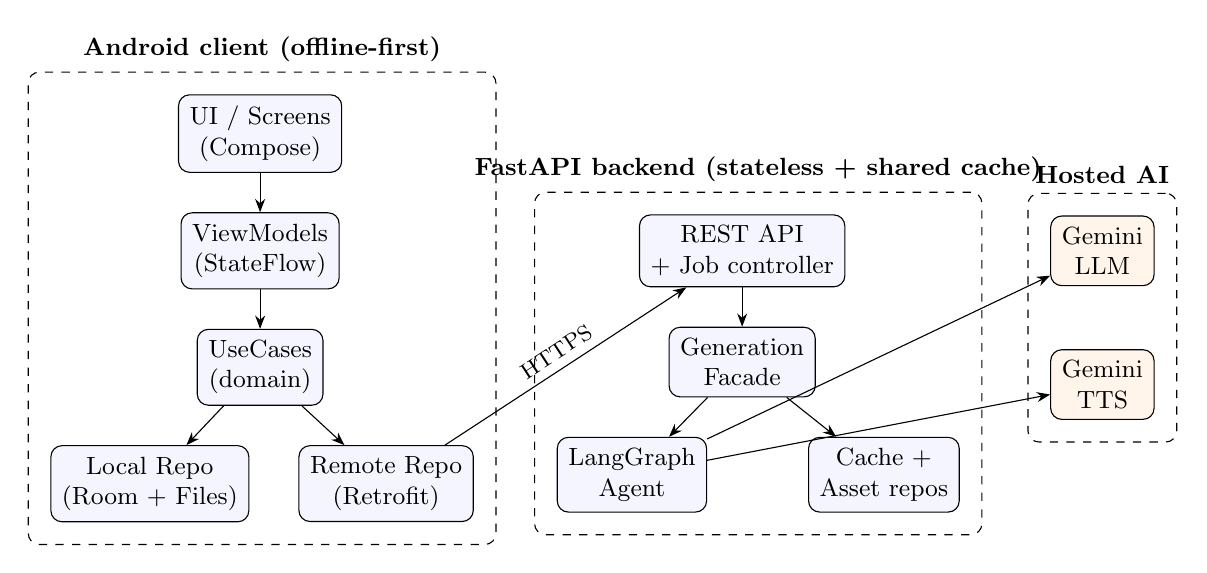
\begin{tikzpicture}[
  font=\small,
  box/.style={draw, rounded corners, align=center, minimum height=8mm,
              inner sep=4pt, fill=blue!4},
  ext/.style={draw, rounded corners, align=center, minimum height=8mm,
              inner sep=4pt, fill=orange!8},
  grp/.style={draw, dashed, rounded corners, inner sep=8pt},
  >={Stealth}
]
% Client column
\node[box] (ui)   {UI / Screens\\(Compose)};
\node[box, below=5mm of ui]   (vm)  {ViewModels\\(StateFlow)};
\node[box, below=5mm of vm]   (uc)  {UseCases\\(domain)};
\node[box, below=5mm of uc, xshift=-14mm] (local) {Local Repo\\(Room + Files)};
\node[box, below=5mm of uc, xshift=16mm]  (remote){Remote Repo\\(Retrofit)};

\begin{scope}[on background layer]
\node[grp, fit=(ui)(vm)(uc)(local)(remote), label=above:{\textbf{Android client (offline-first)}}] (client) {};
\end{scope}

% Backend column
\node[box, right=38mm of vm] (rest) {REST API\\+ Job controller};
\node[box, below=5mm of rest] (facade) {Generation\\Facade};
\node[box, below=5mm of facade, xshift=-14mm] (graph) {LangGraph\\Agent};
\node[box, below=5mm of facade, xshift=18mm]  (cache) {Cache +\\Asset repos};

\begin{scope}[on background layer]
\node[grp, fit=(rest)(facade)(graph)(cache), label=above:{\textbf{FastAPI backend (stateless + shared cache)}}] (backend) {};
\end{scope}

% External column
\node[ext, right=26mm of rest] (llm) {Gemini\\LLM};
\node[ext, below=8mm of llm] (tts) {Gemini\\TTS};

\begin{scope}[on background layer]
\node[grp, fit=(llm)(tts), label=above:{\textbf{Hosted AI}}] (ai) {};
\end{scope}

% edges
\draw[->] (ui) -- (vm);
\draw[->] (vm) -- (uc);
\draw[->] (uc) -- (local);
\draw[->] (uc) -- (remote);
\draw[->] (remote) -- node[above, sloped, font=\footnotesize]{HTTPS} (rest);
\draw[->] (rest) -- (facade);
\draw[->] (facade) -- (graph);
\draw[->] (facade) -- (cache);
\draw[->] (graph) -- (llm);
\draw[->] (graph) -- (tts);
\end{tikzpicture}
\caption{System architecture. A thin offline-first Android client talks to a
stateless FastAPI backend over HTTPS. The backend orchestrates hosted AI
through swappable provider adapters and serves repeated topics from a shared
cache.}
\label{fig:arch}
\end{figure}

In deployment terms, the backend runs as a single container (Uvicorn +
FastAPI) whose generation work executes as asynchronous background tasks; the
lesson cache and asset store run, per configuration, either in memory, on the
filesystem, or against a database and object storage. The interfaces are
identical across these profiles, so promotion from the development profile to
a separate worker with cloud storage requires no call-site changes. The
production instance is deployed on a cloud virtual machine behind an
auto-HTTPS reverse proxy (Section~\ref{sec:infra}).

%------------------------------------------------------------------------------
\section{Domain Model and Lesson Manifest}
\label{sec:domainmodel}
%------------------------------------------------------------------------------

\subsection{Core Entities}

The backend's domain layer defines two central entities.

A \textbf{Lesson} carries an identifier, the original topic and its
normalized \texttt{topic\_key}, a display title, language and voice
parameters, the SVG document, the ordered list of segments, the total
duration, and a creation timestamp. A \textbf{Segment} carries its index, the
narration text, the list of SVG element identifiers it references, a
reference to its audio asset, and its measured duration in milliseconds.

Four invariants are enforced on these entities:

\begin{enumerate}
  \item \texttt{Lesson.svg} is well-formed XML with a \texttt{viewBox};
  \item every value in \texttt{Segment.svg\_element\_ids} exists as an
        \texttt{id} in \texttt{Lesson.svg};
  \item $\texttt{total\_duration\_ms} = \sum_i \texttt{duration\_ms}_i$; and
  \item segments are contiguous and ordered by index starting at 0.
\end{enumerate}

Invariants (1) and (2) are exactly what the deterministic gate of
Section~\ref{sec:gate} checks; (3) and (4) are established by the assembler.

\subsection{The Lesson Manifest}

The manifest is the wire and storage contract shared by the API and the
device (Listing~\ref{lst:manifest}). Asset URLs are downloadable; after
download the device rewrites them to local file paths, which is what makes
offline replay a non-event.

\begin{figure}[htbp]
\begin{lstlisting}[style=code,
  caption={Lesson manifest (abridged): the wire and storage contract.},
  label={lst:manifest}]
{
  "id": "les_8f3a...",
  "topic": "Photosynthesis",
  "title": "How Photosynthesis Works",
  "language": "en",
  "voice": "en-US-neutral",
  "total_duration_ms": 41200,
  "svg": { "asset_id": "ast_svg_01", "url": ".../assets/ast_svg_01" },
  "segments": [
    {
      "index": 0,
      "text": "Sunlight strikes the leaf and is captured by the plant.",
      "svg_element_ids": ["sun", "leaf"],
      "audio": { "asset_id": "ast_aud_00", "url": ".../assets/ast_aud_00" },
      "duration_ms": 4200
    },
    {
      "index": 1,
      "text": "Chlorophyll inside the chloroplasts absorbs that light energy.",
      "svg_element_ids": ["chloroplast", "chlorophyll"],
      "audio": { "asset_id": "ast_aud_01", "url": ".../assets/ast_aud_01" },
      "duration_ms": 3100
    }
  ]
}
\end{lstlisting}
\end{figure}

\subsection{Persistence Schemas}

On the backend, three stores back the service: \texttt{CACHED\_LESSON}
(keyed by \texttt{topic\_key}, holding the manifest and a hit counter),
\texttt{GENERATION\_JOB} (job id, topic key, status, progress, resulting
lesson id or error), and \texttt{ASSET} (asset id, kind
$\in\{\texttt{svg},\texttt{audio}\}$, content type, storage path). On the
device, Room stores \texttt{LESSON\_ENTITY} (metadata plus local SVG path)
and \texttt{SEGMENT\_ENTITY} (text, JSON-encoded identifier list, local
audio path, duration), while the binary assets live in app-private files.

%------------------------------------------------------------------------------
\section{Backend Implementation}
\label{sec:backendimpl}
%------------------------------------------------------------------------------

The backend is a Python FastAPI application of roughly two thousand lines,
organized by responsibility:

\begin{itemize}
  \item \texttt{app/api} --- routers and dependency wiring;
  \item \texttt{app/core} --- typed settings, logging, error envelope;
  \item \texttt{app/domain} --- entities, value objects, Pydantic schemas;
  \item \texttt{app/agents} --- the LangGraph graph and prompts;
  \item \texttt{app/providers} --- LLM and TTS adapters (mock and Gemini);
  \item \texttt{app/services} --- the generation facade and assembler; and
  \item \texttt{app/repositories} --- lesson cache and asset stores.
\end{itemize}

A single composition root wires these together, so swapping any
implementation happens in one place plus the typed settings object.

\subsection{Configuration over Hard-Coding}

Everything that varies between environments is read from environment
variables through one typed settings object, following the twelve-factor
configuration guideline~\cite{twelvefactor}: the choice of LLM and TTS
provider (mock or Gemini), the generation engine, the model identifiers, the
storage backend (memory or filesystem), and the loop budgets $K$ and $R$.
Model identifiers deserve emphasis: hosted model names change over time, so
they are configuration, not code. A small helper
(\texttt{python -m app.tools.list\_models}) lists the live models so the
pinned name can be confirmed; at the time of writing the backend is pinned to
a Flash-class Gemini text model (\texttt{gemini-2.5-flash}) and a Flash-class
Gemini speech model, both set in settings. The same codebase runs on mock or
real providers depending only on settings --- the property that keeps the
test suite fast and key-free.

\subsection{Provider Adapters}

Two narrow interfaces define what the pipeline needs. The \texttt{LLMProvider}
can plan concepts, draw an SVG, critique and refine an SVG, write narration
as structured data, and repair a drawing-plus-narration given an error list.
The \texttt{TTSProvider} turns text into an audio clip and reports its
duration. Each has two implementations:

\begin{itemize}
  \item \textbf{Mock providers} are deterministic and need no network ---
        ideal for tests and local development.
  \item \textbf{Gemini providers} call the hosted models through the
        \texttt{google-genai} SDK, using schema-constrained structured output
        for plans, narration, and repairs. The TTS adapter receives raw PCM
        audio, wraps it as a WAV file, and computes the exact duration from
        the byte count and sample rate --- the duration is a measured fact,
        not an estimate. Both adapters retry transient errors with
        exponential backoff.
\end{itemize}

A provider factory builds a coherent set of providers from settings
(abstract factory), and the generation facade
(\texttt{LessonGenerationFacade}) exposes one entry point that checks the
cache, runs the graph if needed, and persists the result.

\subsection{The Generation Graph in Code}

The pipeline of Section~\ref{sec:genmethod} is implemented as a LangGraph
\texttt{StateGraph} over a typed state object whose fields are set
progressively by the nodes: \texttt{topic} and \texttt{options} at entry;
\texttt{plan} by the planner; \texttt{svg} by the generator and refiner;
\texttt{segments} by the narration generator and repairer;
\texttt{validation} by the validator; \texttt{retries} by the repair loop;
\texttt{rendered} (audio plus durations) by the TTS renderer; \texttt{lesson}
by the assembler; and \texttt{error} by any node on hard failure. Conditional
edges route on the critique score and the validation verdict, with both loops
bounded by settings. Because the graph drives the provider \emph{interfaces},
the identical graph runs on mocks in tests and on Gemini in production.

%------------------------------------------------------------------------------
\section{API Design}
\label{sec:apidesign}
%------------------------------------------------------------------------------

The API is JSON over HTTPS under a versioned base path (\texttt{/api/v1}).
Generation is asynchronous because a cold lesson takes seconds, while cache
hits return immediately. Table~\ref{tab:api} lists the endpoints.

\begin{table}[htbp]
\caption{REST API endpoints}
\label{tab:api}
\centering
\small
\renewcommand{\arraystretch}{1.3}
\begin{tabular}{@{}llp{0.30\textwidth}p{0.24\textwidth}@{}}
\toprule
\textbf{Method} & \textbf{Path} & \textbf{Purpose} & \textbf{Success}\\
\midrule
POST & \texttt{/lessons} & Request a lesson for a topic & 200 (cache hit,
manifest) or 202 (job started)\\
GET & \texttt{/lessons/jobs/\{id\}} & Poll job status & 200 (status,
progress, stage)\\
GET & \texttt{/lessons/\{id\}} & Fetch a lesson manifest & 200 (manifest)\\
GET & \texttt{/assets/\{id\}} & Download an asset (SVG/audio) & 200 (bytes)\\
GET & \texttt{/healthz} & Liveness/readiness & 200\\
\bottomrule
\end{tabular}
\end{table}

A job response reports \texttt{status} $\in$ \{\texttt{queued},
\texttt{running}, \texttt{succeeded}, \texttt{failed}\}, a progress
percentage, and the current pipeline stage (\texttt{planning},
\texttt{svg}, \texttt{narration}, \texttt{validating},
\texttt{tts\_rendering}, \texttt{assembling}), which the client surfaces in
its progress UI. All errors share one envelope --- a machine-readable
\texttt{code} (for example \texttt{INVALID\_TOPIC},
\texttt{GENERATION\_FAILED}, \texttt{PROVIDER\_UNAVAILABLE}), a human
message, a \texttt{retryable} flag, and a correlation \texttt{request\_id}
--- so the client has exactly one error-handling path.
\texttt{POST /lessons} is idempotent per topic key, and concurrent identical
requests coalesce onto a single job (Section~\ref{sec:cachemethod}).

%------------------------------------------------------------------------------
\section{Android Client Implementation}
\label{sec:clientimpl}
%------------------------------------------------------------------------------

The client is a Kotlin application of roughly 3\,800 lines using Jetpack
Compose, structured by Clean Architecture~\cite{martin2017clean} into three
layers with dependencies pointing inward:

\begin{itemize}
  \item \textbf{Presentation} --- Compose screens (Topic, Player, History)
        and ViewModels that expose a single immutable \texttt{UiState} via
        \texttt{StateFlow}; the UI is a pure function of state.
  \item \textbf{Domain} --- pure Kotlin use cases (generate lesson, get
        history, play lesson, delete lesson), entities, and repository
        interfaces; no Android dependencies.
  \item \textbf{Data} --- a remote repository (Retrofit) implementing
        generation and download against the API, and a local repository
        (Room + file store) implementing persistence; both implement the
        domain's interfaces (dependency inversion).
\end{itemize}

Dependency injection is performed by a small manual composition root
(\texttt{AppContainer}); this was a deliberate deviation from the initial
Hilt plan, chosen for build reliability, and is swappable later since the
seams are the repository interfaces.

\subsection{Generation Flow on the Device}

The Topic screen submits the topic and then polls the job endpoint with
backoff, rendering the reported stage and progress. On success it fetches the
manifest and hands it to the player. Errors surface the envelope's message
with a retry affordance (FR-12).

\subsection{Synchronized Playback}

The player is the product's core (Figure~\ref{fig:player}). Two components
cooperate:

\begin{itemize}
  \item \textbf{Highlight engine.} The SVG is rendered in a WebView as an
        inline document together with a small app-owned script exposing
        \texttt{highlight(ids)} and \texttt{clearHighlight()}, which toggle a
        CSS class producing a glow-and-scale emphasis. The WebView renders
        \emph{only} this app-generated page; generated SVG is treated as
        untrusted markup and no content-supplied script is executed.
  \item \textbf{Segment clock.} ExoPlayer is loaded with one media item per
        segment clip, in order. The player's current-item index \emph{is} the
        synchronization state: on each transition to item $i$, the ViewModel
        highlights $E_i$ and updates the caption to the segment text.
\end{itemize}

Transport controls (previous, play/pause, next, replay) map onto playlist
operations, and the player follows the state machine
Idle $\to$ Loading $\to$ Ready $\to$ Playing $\rightleftharpoons$ Paused, with
Seeking, Completed (replay returns to Playing), and Error (retry returns to
Loading) states.

\begin{figure}[htbp]
\centering
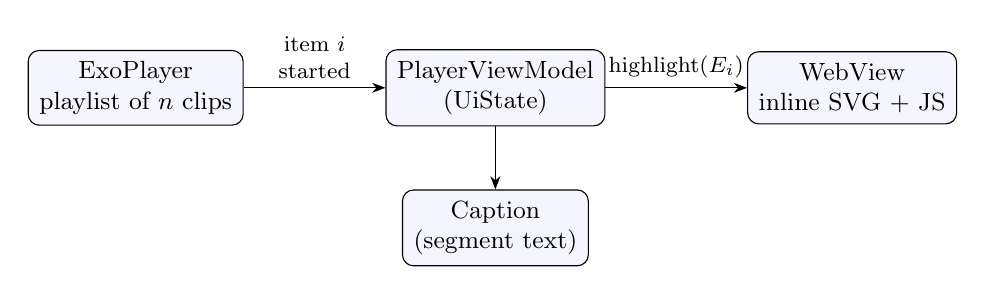
\begin{tikzpicture}[
  font=\small,
  n/.style={draw, rounded corners, align=center, minimum height=8mm,
            inner sep=4pt, fill=blue!4},
  >={Stealth}
]
\node[n] (exo) {ExoPlayer\\playlist of $n$ clips};
\node[n, right=18mm of exo] (vmn) {PlayerViewModel\\(UiState)};
\node[n, right=18mm of vmn] (web) {WebView\\inline SVG + JS};
\node[n, below=8mm of vmn] (cap) {Caption\\(segment text)};

\draw[->] (exo) -- node[above,font=\footnotesize,align=center]
  {item $i$\\started} (vmn);
\draw[->] (vmn) -- node[above,font=\footnotesize,align=center]
  {highlight($E_i$)} (web);
\draw[->] (vmn) -- (cap);
\end{tikzpicture}
\caption{Synchronized playback. The audio player's current-item index drives
both the SVG highlight and the caption; no other timing state exists.}
\label{fig:player}
\end{figure}

\subsection{Offline Persistence and History}

``Save offline'' downloads the SVG and every audio clip into app-private
files and persists lesson and segment rows in Room; manifest asset URLs are
rewritten to local file URIs. The player is source-agnostic --- it receives a
loader function, so a saved lesson loads from local URIs through exactly the
same code path as a fresh one, and replays with zero network calls (NFR-2).
The History screen observes Room reactively (newest first); delete removes
both the rows and the files. History never leaves the device (NFR-7).

%------------------------------------------------------------------------------
\section{Design Patterns at the Seams}
\label{sec:patterns}
%------------------------------------------------------------------------------

Table~\ref{tab:patterns} maps the classical patterns~\cite{gamma1994} to
their locations and purposes in the system. The common motivation is
\emph{soft dependencies}: every external or replaceable concern sits behind
an interface chosen once, in one place.

\begin{table}[htbp]
\caption{Design patterns employed}
\label{tab:patterns}
\centering
\small
\renewcommand{\arraystretch}{1.3}
\begin{tabular}{@{}lp{0.34\textwidth}p{0.38\textwidth}@{}}
\toprule
\textbf{Pattern} & \textbf{Where} & \textbf{Why}\\
\midrule
Strategy & \texttt{LLMProvider}, \texttt{TTSProvider} & Swap AI vendors
without touching the graph\\
Abstract Factory & \texttt{ProviderFactory} & Build a coherent provider set
from configuration\\
Adapter & Gemini LLM/TTS classes & Wrap vendor SDKs behind the project's
interfaces\\
Builder & \texttt{LessonBuilder} & Assemble a valid \texttt{Lesson}
incrementally\\
Repository & Lesson cache, asset store, Android repositories & Hide storage
behind interfaces; memory/filesystem/DB profiles\\
Facade & \texttt{LessonGenerationFacade} & One entry point over cache check,
graph, and persistence\\
Pipeline & LangGraph nodes and conditional edges & Staged generation with
bounded loops\\
DTO & Pydantic schemas; manifest & Typed boundaries between layers and over
the wire\\
Dependency Injection & FastAPI wiring; \texttt{AppContainer} & Testability;
single composition root\\
Observer & \texttt{StateFlow} UiState; Room \texttt{Flow} & Reactive UI as a
pure function of state\\
\bottomrule
\end{tabular}
\end{table}

%------------------------------------------------------------------------------
\section{Hermetic Testing, Containerization, and CI/CD}
\label{sec:infra}
%------------------------------------------------------------------------------

\subsection{Hermetic, Key-Free Tests}

The backend suite comprises 48 tests covering the validator (both accepting
and rejecting), each graph node, the repair loop (recovery and
exhausted-budget failure), the API contract including the error envelope, the
job model, the repositories, and the Gemini adapters via a faked SDK client.
A session-level fixture disables \texttt{.env} loading and strips all
\texttt{TUTOR\_*} environment variables, so the suite is deterministic,
requires no secrets, and makes zero live API calls --- in any clone and in
CI.

\subsection{Containerization and Continuous Delivery}

The backend ships as a Docker image with a \texttt{/healthz} healthcheck and
a Compose profile for local orchestration. Four GitHub Actions workflows
automate the path from commit to artifact:

\begin{enumerate}
  \item \textbf{backend-ci} --- runs the hermetic test suite and builds the
        Docker image on every push;
  \item \textbf{backend-deploy} --- publishes the image to a container
        registry and deploys it over SSH to the cloud host, where an
        auto-HTTPS reverse proxy terminates TLS;
  \item \textbf{android-ci} --- assembles a debug APK as a build artifact;
        and
  \item \textbf{android-release} --- produces a signed release APK and
        attaches it to a GitHub Release, with a debug-key fallback when no
        signing secret is configured.
\end{enumerate}

Together with configuration-through-environment, this makes the entire system
reproducible: a fresh clone can run the full test suite with no keys, and a
tagged commit yields both a deployable backend image and an installable
client build with no manual steps.

%==============================================================================
\chapter{Results and Discussion}
\label{ch:results}
%==============================================================================

This chapter reports what the running system produces and what was verified,
and is explicit about what has not yet been measured. The claims below are
about the realized system's observed behaviour; no user-study or
learning-outcome figures are reported, because none were collected.

%------------------------------------------------------------------------------
\section{Results and Analysis}
\label{sec:results}
%------------------------------------------------------------------------------

\subsection{End-to-End Generation Against Live Models}

With the real Gemini providers configured, the pipeline produced a complete
lesson for the topic \emph{Photosynthesis}: six narration segments totalling
approximately forty-three seconds of audio, a well-formed SVG whose parts
carry semantic identifiers such as \texttt{sun}, \texttt{leaf}, and
\texttt{chloroplast}, narration whose references all passed the
deterministic validator, and real synthesized speech for each segment. This
single run exercises every node of the graph --- planner, SVG generator,
critique/refine, narration generator, validator, TTS renderer, and assembler
--- against live models. Figure~\ref{fig:diagram} shows the generated
diagram as rendered by the app.

\begin{figure}[htbp]
\centering
\shot[width=0.85\textwidth]{diagram.png}
\caption{The diagram generated for \emph{Photosynthesis}, as shown in the
app's full-screen view. Each labelled part --- the sun, the leaf, the
chloroplast, the water and carbon-dioxide inputs, and the glucose and oxygen
outputs --- is a separate SVG element with a stable identifier, which is
exactly what lets the narration highlight it during playback.}
\label{fig:diagram}
\end{figure}

The saved library shown in Figure~\ref{fig:screens} holds further lessons
generated for unrelated topics --- the Pythagorean theorem and the
Transformer architecture --- demonstrating that the pipeline is not tuned to
a single subject: the same prompts, graph, and validator produced consistent
lessons across a natural-science topic, a mathematical topic, and a
computer-science topic.

\begin{figure}[htbp]
\centering
\begin{tabular}{ccc}
\shot[width=0.30\textwidth]{home.png} &
\shot[width=0.30\textwidth]{player.png} &
\shot[width=0.30\textwidth]{library.png}\\
(a) Topic entry & (b) Player & (c) Library\\
\end{tabular}
\caption{The Android client. (a)~The home screen where a topic is typed.
(b)~The player mid-lesson: the current segment's diagram parts are
highlighted while its audio plays, with the caption below. (c)~The on-device
library of saved lessons, each replayable fully offline.}
\label{fig:screens}
\end{figure}

\subsection{The Validation Gate Works in Both Directions}

The property the design promises is that the gate both catches broken
lessons and does not block valid ones. Both directions were verified by the
graph tests:

\begin{itemize}
  \item a lesson containing a deliberately broken part reference is
        \emph{rejected} by the validator and routed into the repair loop,
        and when the repair succeeds the corrected lesson passes and
        proceeds to rendering; and
  \item when repair cannot fix the problem within the retry budget $R$, the
        job \emph{fails cleanly} --- no partial or inconsistent lesson is
        ever cached.
\end{itemize}

Combined with the live run above (where valid generations passed the gate
unimpeded), this confirms the system-wide invariant: every lesson that
reaches the cache satisfies ``all referenced identifiers exist.''

\subsection{Synchronization Behaviour}

Because each segment's duration is computed from the synthesized audio's
byte count and sample rate, and the on-device highlight is driven by the
audio player's current-item index, the highlight transition coincides with
the clip transition by construction. Playback, pause, resume,
seek-by-segment, and replay all preserve synchronization, since the only
synchronization state is the current clip index. The same behaviour holds
for offline replays, where all assets are local files.

\subsection{Reproducibility and Automation Results}

Table~\ref{tab:verified} summarizes the verification of the engineering
infrastructure.

\begin{table}[htbp]
\caption{Verified engineering results}
\label{tab:verified}
\centering
\small
\renewcommand{\arraystretch}{1.3}
\begin{tabular}{@{}p{0.34\textwidth}p{0.58\textwidth}@{}}
\toprule
\textbf{Aspect} & \textbf{Verified result}\\
\midrule
Backend test suite & 48 hermetic tests pass with \emph{zero} live API calls
and no keys present\\
Container & Docker image builds; container serves \texttt{/healthz} (200);
mock-provider generation returns the expected 202 asynchronous response with
no key\\
Client build & Debug APK assembles reproducibly in CI; release workflow
produces a signed APK\\
Deployment & Backend image published to a registry and deployed to a cloud
host behind auto-HTTPS by the deploy workflow\\
Offline path & Save-offline persists all assets locally; the player loads
saved lessons from local file URIs through the same code path as fresh
lessons\\
Model-id resilience & Live model listing tool confirms pinned identifiers;
changing models is a settings change only\\
\bottomrule
\end{tabular}
\end{table}

\subsection{The Realized System at a Glance}

\begin{table}[htbp]
\caption{Realized system summary}
\label{tab:summary}
\centering
\small
\renewcommand{\arraystretch}{1.3}
\begin{tabular}{@{}ll@{}}
\toprule
\textbf{Aspect} & \textbf{Realization}\\
\midrule
Backend & FastAPI, $\approx$2.0k LoC Python\\
Client & Android/Compose, $\approx$3.8k LoC Kotlin\\
Generation & LangGraph: plan $\to$ draw $\to$ critique/refine $\to$ narrate
$\to$ validate $\to$ repair\\
Gate & Deterministic non-LLM validator\\
Models & Text + speech via swappable adapters (Gemini Flash class)\\
Caching & Stateless, topic-keyed, coalesced jobs\\
Offline & Room + file store; network-free replay\\
Tests & 48 hermetic, key-free backend tests\\
Delivery & Container + CI/CD + auto-HTTPS deployment\\
\bottomrule
\end{tabular}
\end{table}

%------------------------------------------------------------------------------
\section{Discussion}
\label{sec:discussion}
%------------------------------------------------------------------------------

\subsection{Analysis of the Design Choices}

\textbf{The gate, not the model, carries the guarantee.} The central result
of this work is architectural: the correctness-critical property (narration
references resolve) is enforced by a component that cannot hallucinate. The
LLM-facing mechanisms --- planning first, narrating against the finished
drawing, structured output, low temperature --- \emph{reduce the frequency}
of violations, and the repair loop \emph{recovers} from most of the rest,
but the deterministic validator is what converts ``usually consistent'' into
``never served inconsistent.'' This separation of concerns (probabilistic
quality mechanisms in front of a deterministic correctness mechanism) is
transferable to any system whose LLM outputs must satisfy checkable
invariants.

\textbf{Bounded loops keep the worst case owned.} Both self-correction loops
carry explicit budgets, so the maximum number of model calls per lesson is
known in advance, and the failure mode of an unfixable topic is a clean,
retryable error rather than an unbounded spend. This is a deliberate
divergence from open-ended agent designs in the literature.

\textbf{The cache changes the economics.} Statelessness plus topic-keyed
caching means the marginal cost of a popular topic tends to zero and the
response time collapses to a lookup. Request coalescing caps the cost spike
of a suddenly popular topic at one generation.

\subsection{Limitations}

Several limitations are worth naming plainly.

\emph{Diagram quality has a ceiling.} A language model drawing SVG is good
at clear, well-known concepts and weaker at dense or unusual ones. The
critique-and-refine loop raises the floor but does not guarantee a beautiful
result: the deterministic gate guarantees \emph{consistency}, not aesthetic
quality --- a valid lesson can still be a plain one.

\emph{Synchronization is at the segment level.} A group of parts is lit for
a whole sentence, not each part at its spoken word. This was a deliberate
trade for determinism and offline play; word-level highlighting would be
more precise but would reintroduce timing data and fragility.

\emph{Cold topics are slow and cost money.} The first request for a new
topic pays for several model calls and speech synthesis and takes seconds.
The cache hides this for repeated topics and the bounded loops cap the worst
case, but the cold path is inherently the slow path.

\emph{Generated markup must be treated as untrusted.} Rendering
model-produced SVG in a WebView requires care; the WebView is restricted to
the app's own highlight script and content-supplied script is not executed,
but this remains an area demanding ongoing attention.

\emph{Evaluation breadth.} The claims here are about verified system
behaviour, not measured learning gains. No controlled user study, no large
quantitative study of diagram quality across many topics, and no on-device
latency or battery measurements across a fleet of devices have been
performed; these are flagged as future work rather than claimed as results.

%==============================================================================
\chapter{Conclusion and Future Scope}
\label{ch:conclusion}
%==============================================================================

\section{Conclusion}
\label{sec:conclusion}

This thesis presented TutorAI, a complete, working system that turns a typed
topic into a short, self-explaining lesson: a vector diagram whose parts
carry stable semantic identifiers, segment-level narration tied to those
identifiers, and per-segment synthesized audio that drives synchronized
highlighting on an Android device --- fully offline once downloaded, with an
on-device history and no user accounts.

All six objectives set out in Section~\ref{sec:objectives} were met. An
agentic generation pipeline was designed and implemented as a LangGraph state
graph that transforms a free-text topic into a validated lesson
(Objective~1). A deterministic, non-LLM validation gate with bounded
critique-and-refine and repair loops guarantees that no lesson with a broken
narration reference is ever cached or served, and this guarantee was verified
in both directions --- rejection and repair of broken lessons, and clean
failure when repair is exhausted (Objective~2). A stateless FastAPI backend
provides the asynchronous job model, the shared topic-keyed cache with
request coalescing, the asset store, and swappable Gemini provider adapters
(Objective~3). An offline-first Android client built with Jetpack Compose,
Clean Architecture, and MVVM generates lessons via job polling, plays them
with deterministic segment-synchronized highlighting, and persists them for
network-free replay (Objective~4). The engineering practice throughout ---
UML-first design, classical patterns at the seams, 48 hermetic key-free
tests, containerization, and CI/CD for both backend and client --- makes the
system reproducible from a fresh clone (Objective~5). Finally, the realized
system was verified end to end against live models, producing consistent
lessons across topics as different as photosynthesis, the Pythagorean
theorem, and the Transformer architecture (Objective~6).

The central insight of the work is architectural rather than about any
single model. By splitting generation into a small graph of steps, adding a
bounded critique-and-refine loop for the drawing and a bounded repair loop
for the narration, and placing a deterministic, non-LLM validator in front
of the cache, a probabilistic generator is made reliable enough to power a
feature that depends on exact part-to-word correspondence. Around this core,
a stateless caching backend keeps cost down, provider adapters keep the
vendor choice soft, and an offline-first client keeps the lesson usable
without a network. The pattern --- probabilistic quality mechanisms in front
of a deterministic correctness gate --- transfers directly to any
application whose LLM outputs must satisfy machine-checkable invariants.

\section{Future Scope}
\label{sec:futurescope}

Future work falls into three groups; none changes the central design ---
each extends it.

\textbf{Evaluation.} The most important next step is empirical: a controlled
learning study comparing TutorAI lessons against static diagrams and plain
text, grounded in the multimedia-learning predictions that motivated the
product form; a larger automatic study of diagram quality and validator
pass/repair/fail rates across hundreds of topics; and on-device latency,
memory, and energy measurements across a range of phones.

\textbf{Capability.} Several extensions are natural. Optional word-level
highlighting where TTS timing metadata is available, degrading gracefully to
segment-level sync offline. Richer diagram styles and layout hints from the
planner. A research or planning step in front of the drawing (for example, a
retrieval or deep-research agent behind the existing
\texttt{LLMProvider.plan\_concepts} port) for harder or fast-moving topics.
Multi-language lessons --- the manifest already carries language and voice
parameters. Accessibility refinements such as adjustable playback speed and
transcript export.

\textbf{Scale.} The development profile's in-process worker and filesystem
store can be promoted to a separate worker pool, a managed PostgreSQL cache,
and cloud object storage behind the same repository interfaces, with no
call-site changes. Server-sent events can replace job polling. A lightweight
API key can be introduced through the header slot the contract already
reserves, if usage ever warrants it.


% ================================ BACK MATTER =================================
%================================ REFERENCES ==================================
\clearpage
\addcontentsline{toc}{chapter}{References}
\renewcommand{\bibname}{References}

\begin{thebibliography}{00}
\addtolength{\itemsep}{-2pt}

\bibitem{bloom1984} B.~S. Bloom, ``The 2 sigma problem: The search for methods
of group instruction as effective as one-to-one tutoring,'' \emph{Educational
Researcher}, vol.~13, no.~6, pp.~4--16, 1984.

\bibitem{anderson1995cognitive} J.~R. Anderson, A.~T. Corbett, K.~R. Koedinger,
and R.~Pelletier, ``Cognitive tutors: Lessons learned,'' \emph{The Journal of
the Learning Sciences}, vol.~4, no.~2, pp.~167--207, 1995.

\bibitem{vanlehn2011} K.~VanLehn, ``The relative effectiveness of human
tutoring, intelligent tutoring systems, and other tutoring systems,''
\emph{Educational Psychologist}, vol.~46, no.~4, pp.~197--221, 2011.

\bibitem{kasneci2023chatgpt} E.~Kasneci \emph{et al.}, ``ChatGPT for good? On
opportunities and challenges of large language models for education,''
\emph{Learning and Individual Differences}, vol.~103, 102274, 2023.

\bibitem{paivio1991} A.~Paivio, ``Dual coding theory: Retrospect and current
status,'' \emph{Canadian Journal of Psychology}, vol.~45, no.~3, pp.~255--287,
1991.

\bibitem{sweller1988} J.~Sweller, ``Cognitive load during problem solving:
Effects on learning,'' \emph{Cognitive Science}, vol.~12, no.~2, pp.~257--285,
1988.

\bibitem{mayer2014multimedia} R.~E. Mayer, Ed., \emph{The Cambridge Handbook of
Multimedia Learning}, 2nd~ed. Cambridge, U.K.: Cambridge Univ. Press, 2014.

\bibitem{mayermoreno2003} R.~E. Mayer and R.~Moreno, ``Nine ways to reduce
cognitive load in multimedia learning,'' \emph{Educational Psychologist},
vol.~38, no.~1, pp.~43--52, 2003.

\bibitem{vaswani2017attention} A.~Vaswani \emph{et al.}, ``Attention is all you
need,'' in \emph{Proc. Advances in Neural Information Processing Systems
(NeurIPS)}, 2017, pp.~5998--6008.

\bibitem{brown2020gpt3} T.~B. Brown \emph{et al.}, ``Language models are
few-shot learners,'' in \emph{Proc. Advances in Neural Information Processing
Systems (NeurIPS)}, 2020, pp.~1877--1901.

\bibitem{gemini2023} Gemini Team, Google, ``Gemini: A family of highly capable
multimodal models,'' arXiv:2312.11805, 2023.

\bibitem{chen2021codex} M.~Chen \emph{et al.}, ``Evaluating large language
models trained on code,'' arXiv:2107.03374, 2021.

\bibitem{liu2023promptsurvey} P.~Liu \emph{et al.}, ``Pre-train, prompt, and
predict: A systematic survey of prompting methods in natural language
processing,'' \emph{ACM Computing Surveys}, vol.~55, no.~9, pp.~1--35, 2023.

\bibitem{ji2023hallucination} Z.~Ji \emph{et al.}, ``Survey of hallucination in
natural language generation,'' \emph{ACM Computing Surveys}, vol.~55, no.~12,
pp.~1--38, 2023.

\bibitem{rombach2022stable} R.~Rombach, A.~Blattmann, D.~Lorenz, P.~Esser, and
B.~Ommer, ``High-resolution image synthesis with latent diffusion models,'' in
\emph{Proc. IEEE/CVF Conf. Computer Vision and Pattern Recognition (CVPR)},
2022, pp.~10684--10695.

\bibitem{wei2022cot} J.~Wei \emph{et al.}, ``Chain-of-thought prompting elicits
reasoning in large language models,'' in \emph{Proc. Advances in Neural
Information Processing Systems (NeurIPS)}, 2022.

\bibitem{yao2023react} S.~Yao \emph{et al.}, ``ReAct: Synergizing reasoning and
acting in language models,'' in \emph{Proc. Int. Conf. Learning Representations
(ICLR)}, 2023.

\bibitem{madaan2023selfrefine} A.~Madaan \emph{et al.}, ``Self-Refine: Iterative
refinement with self-feedback,'' in \emph{Proc. Advances in Neural Information
Processing Systems (NeurIPS)}, 2023.

\bibitem{shinn2023reflexion} N.~Shinn \emph{et al.}, ``Reflexion: Language
agents with verbal reinforcement learning,'' in \emph{Proc. Advances in Neural
Information Processing Systems (NeurIPS)}, 2023.

\bibitem{chen2023selfdebug} X.~Chen, M.~Lin, N.~Sch\"arli, and D.~Zhou,
``Teaching large language models to self-debug,'' arXiv:2304.05128, 2023.

\bibitem{langchain} H.~Chase, ``LangChain,'' open-source software, 2022.
[Online]. Available: \url{https://github.com/langchain-ai/langchain}

\bibitem{langgraph} LangChain, ``LangGraph: Building stateful, multi-actor
applications with LLMs,'' software documentation. [Online]. Available:
\url{https://langchain-ai.github.io/langgraph/}

\bibitem{svgspec} World Wide Web Consortium (W3C), ``Scalable Vector Graphics
(SVG) 1.1 (Second Edition),'' W3C Recommendation, 2011. [Online]. Available:
\url{https://www.w3.org/TR/SVG11/}

\bibitem{carlier2020deepsvg} A.~Carlier, M.~Danelljan, A.~Alahi, and
R.~Timofte, ``DeepSVG: A hierarchical generative network for vector graphics
animation,'' in \emph{Proc. Advances in Neural Information Processing Systems
(NeurIPS)}, 2020.

\bibitem{rodriguez2023starvector} J.~A. Rodriguez \emph{et al.}, ``StarVector:
Generating scalable vector graphics code from images,'' arXiv:2312.11556, 2023.

\bibitem{oord2016wavenet} A.~van den Oord \emph{et al.}, ``WaveNet: A generative
model for raw audio,'' arXiv:1609.03499, 2016.

\bibitem{shen2018tacotron2} J.~Shen \emph{et al.}, ``Natural TTS synthesis by
conditioning WaveNet on mel spectrogram predictions,'' in \emph{Proc. IEEE Int.
Conf. Acoustics, Speech and Signal Processing (ICASSP)}, 2018, pp.~4779--4783.

\bibitem{offlinefirst} A.~Feyerke, ``Designing offline-first web apps,'' \emph{A
List Apart}, no.~373, 2013. [Online]. Available:
\url{https://alistapart.com/article/offline-first/}

\bibitem{androidguide} Google, ``Guide to app architecture,'' Android Developers
documentation. [Online]. Available:
\url{https://developer.android.com/topic/architecture}

\bibitem{martin2017clean} R.~C. Martin, \emph{Clean Architecture: A Craftsman's
Guide to Software Structure and Design}. Boston, MA: Prentice Hall, 2017.

\bibitem{twelvefactor} A.~Wiggins, ``The Twelve-Factor App,'' 2017. [Online].
Available: \url{https://12factor.net/}

\bibitem{gamma1994} E.~Gamma, R.~Helm, R.~Johnson, and J.~Vlissides,
\emph{Design Patterns: Elements of Reusable Object-Oriented Software}. Reading,
MA: Addison-Wesley, 1994.

\end{thebibliography}

%============================ PUBLICATION DETAILS =============================
\clearpage
\chapter*{Publication Details}
\addcontentsline{toc}{chapter}{Publication Details}

The following publication has resulted from this project work:

\begin{enumerate}
  \item \candidatename\ and \guidename, ``TutorAI: An Agentic,
        Validation-Gated Pipeline for Self-Explaining,
        Highlight-Synchronized Visual Lessons on an Offline-First Mobile
        App,'' \todoph{conference name, e.g.\ Proc.\ IEEE International
        Conference on \ldots}, \todoph{location}, \todoph{month year},
        \todoph{status: communicated / accepted / presented / published}.
\end{enumerate}

\todoph{Update the entry above with the final conference details, page
numbers, and DOI once available, and attach the acceptance certificate or
first page of the published paper if your department requires it.}

%============================= PLAGIARISM REPORT ==============================
\clearpage
\chapter*{Plagiarism Report}
\addcontentsline{toc}{chapter}{Plagiarism Report}

The thesis was checked for plagiarism using \todoph{tool name, e.g.\
Turnitin / DrillBit} on \todoph{date}. The overall similarity index reported
was \todoph{XX}\%, which is within the limit prescribed by the university.

\vspace{8mm}
\noindent\todoph{Insert the summary page of the plagiarism report here, e.g.:}

% \begin{center}
% \includegraphics[width=0.9\textwidth]{plagiarism-report.png}
% \end{center}

\vspace{20mm}
\noindent
\begin{tabular}{@{}p{0.48\textwidth}p{0.48\textwidth}@{}}
\textbf{\candidatename} & \textbf{\guidename}\\
Candidate & Guide\\
\end{tabular}


\appendix
% Appendix chapter headings read "APPENDIX A" etc.
\renewcommand{\chaptertitlename}{Appendix}
%============================ APPENDIX A: API =================================
\chapter{API Contract and Schemas}
\label{app:api}

\section{Endpoints}

Base path: \texttt{/api/v1}, JSON over HTTPS. See Table~\ref{tab:api} for
the endpoint summary; the request and response bodies are reproduced here.

\subsection*{POST /lessons --- request}
\begin{lstlisting}[style=code]
{
  "topic": "Photosynthesis",
  "language": "en",
  "voice": "en-US-neutral"
}
\end{lstlisting}

\subsection*{POST /lessons --- 202 (generation started)}
\begin{lstlisting}[style=code]
{
  "job_id": "job_3c1...",
  "status": "queued",
  "topic_key": "photosynthesis|en"
}
\end{lstlisting}

A \texttt{200} response (cache hit) returns the full lesson manifest of
Listing~\ref{lst:manifest} instead.

\subsection*{GET /lessons/jobs/\{job\_id\} --- 200}
\begin{lstlisting}[style=code]
{
  "job_id": "job_3c1...",
  "status": "running",
  "progress": 60,
  "stage": "tts_rendering",
  "lesson_id": null,
  "error": null
}
\end{lstlisting}

\texttt{status} $\in$ \{\texttt{queued}, \texttt{running},
\texttt{succeeded}, \texttt{failed}\}; \texttt{stage} $\in$
\{\texttt{planning}, \texttt{svg}, \texttt{narration},
\texttt{validating}, \texttt{tts\_rendering}, \texttt{assembling}\}.

\section{Error Envelope}

All errors share one shape:

\begin{lstlisting}[style=code]
{
  "error": {
    "code": "GENERATION_FAILED",
    "message": "Could not produce a valid diagram for this topic.",
    "retryable": true,
    "request_id": "req_9a2..."
  }
}
\end{lstlisting}

\begin{table}[htbp]
\caption{Error codes}
\label{tab:errors}
\centering
\small
\renewcommand{\arraystretch}{1.3}
\begin{tabular}{@{}clp{0.50\textwidth}@{}}
\toprule
\textbf{HTTP} & \textbf{Code} & \textbf{When}\\
\midrule
400 & \texttt{INVALID\_TOPIC} & Empty, too long, or unsupported characters\\
404 & \texttt{LESSON\_NOT\_FOUND} / \texttt{JOB\_NOT\_FOUND} & Unknown id\\
422 & \texttt{VALIDATION\_ERROR} & Malformed request body\\
429 & \texttt{RATE\_LIMITED} & Too many requests\\
500 & \texttt{GENERATION\_FAILED} & Graph exhausted repair retries or
provider error\\
503 & \texttt{PROVIDER\_UNAVAILABLE} & Upstream AI API down\\
\bottomrule
\end{tabular}
\end{table}

\section{Conventions}

Versioning is path-based (\texttt{/api/v1}); breaking changes move to
\texttt{/v2}. \texttt{POST /lessons} is idempotent per topic key: repeated
requests return the same job or the same cached lesson. Asset URLs are
scoped and time-limited; the device downloads each asset once and thereafter
uses local paths. No authentication exists in version~1 (there are no
accounts); a header slot is reserved for a future API key.

%========================= APPENDIX B: REPOSITORY =============================
\chapter{Repository Layout and Verification Artifacts}
\label{app:repo}

\section{Repository Layout}

\begin{lstlisting}[style=code]
tutor/
|-- README.md
|-- docs/                  # design set (UML): vision, architecture,
|                          # domain model, agent design, sequences,
|                          # API contract, Android architecture, SDLC
|-- backend/               # FastAPI + LangGraph service
|   |-- app/
|   |   |-- api/           # routers, dependencies
|   |   |-- core/          # config (typed Settings), logging, errors
|   |   |-- domain/        # entities, value objects, schemas
|   |   |-- agents/        # LangGraph graph, nodes, prompts
|   |   |-- providers/     # LLM + TTS adapters (mock + Gemini)
|   |   |-- services/      # generation facade, assembler
|   |   |-- repositories/  # lesson cache + asset store
|   |   `-- tools/         # list_models helper
|   |-- tests/             # 48 hermetic, key-free tests
|   |-- Dockerfile
|   `-- docker-compose.yml
|-- android/               # Kotlin + Compose client
|   `-- app/src/main/...   # ui/ (topic, player, history),
|                          # domain/, data/ (remote, local)
`-- .github/workflows/     # backend-ci, backend-deploy,
                           # android-ci, android-release
\end{lstlisting}

\section{Backend Test Coverage Summary}

The 48-test hermetic suite covers, by area:

\begin{itemize}
  \item \textbf{Validator} --- accepts valid SVG/segments; rejects malformed
        XML, missing \texttt{viewBox}, unknown identifiers, empty and
        non-contiguous segments.
  \item \textbf{Generation graph} --- happy path from mock providers;
        repair-loop recovery after an injected broken reference; clean
        failure when the retry budget is exhausted.
  \item \textbf{API contract} --- request/response schemas for all
        endpoints; 200-versus-202 cache behaviour; the error envelope for
        each error code; job lifecycle.
  \item \textbf{Repositories} --- memory and filesystem lesson/asset stores,
        including round-tripping manifests and assets.
  \item \textbf{Gemini adapters} --- structured-output handling, PCM-to-WAV
        wrapping with byte-derived durations, and retry/backoff, exercised
        against a faked SDK client (no network, no keys).
  \item \textbf{Configuration} --- provider/engine/storage selection from
        settings; the session fixture that strips environment variables and
        disables \texttt{.env} loading.
\end{itemize}

\section{Continuous Integration Workflows}

\begin{table}[htbp]
\caption{GitHub Actions workflows}
\label{tab:ci}
\centering
\small
\renewcommand{\arraystretch}{1.3}
\begin{tabular}{@{}lp{0.28\textwidth}p{0.44\textwidth}@{}}
\toprule
\textbf{Workflow} & \textbf{Trigger} & \textbf{Action}\\
\midrule
\texttt{backend-ci} & Push / pull request & Run the hermetic pytest suite;
build the Docker image\\
\texttt{backend-deploy} & Manual / tag & Push image to the container
registry; deploy over SSH to the cloud host (auto-HTTPS proxy)\\
\texttt{android-ci} & Push / pull request & Assemble the debug APK and
upload it as an artifact\\
\texttt{android-release} & Tag & Build a signed release APK and attach it to
a GitHub Release (debug-key fallback)\\
\bottomrule
\end{tabular}
\end{table}


\end{document}
